\chapter{An API for feedback control}
\label{chap:feedback-api}
While studying the principles of feedback control, we discovered that there are hardly any publicly available libraries or APIs that abstract over the notions of feedback control, allowing us to create and execute feedback systems, both in simulation and in practice. Although surprising at first, this is completely in accordance with the earlier observation that feedback control is not (yet) a commonly used technique in computer science\footnote{Even though we were not able to find existing APIs for this purpose, we would not be surprised if companies turned out to have libraries like this in private.}. Surely, we can write the code ourselves as shown in \Cref{sec:imperative-balltracker}, but that isn't really reusable, creates the danger of copy-paste behavior and is more prone to bugs than a dedicated API.

In this chapter we present our own API for creating and executing feedback systems that can potentially be used in production software. \todo{rest of the introduction and layout of this chapter}

\section{Related work}
One of the few libraries we found is described by Philip Janert in his book ``\textit{Feedback Control for Computer Systems}'' \cite{janert2013-feedback}. Janert presents a small framework for simulating feedback loops with the purpose of being a teaching tool that makes it simple and transparent to demonstrate the algorithms presented in several case studies and to encourage experimentation. He explicitly states that little emphasis was placed on elegant implementations or time efficiency and that this framework is not meant to be used in production software. What distinguishes his framework from other simulation frameworks for control systems (for example MatLab \cite{Matlab-Feedback}), however, is the way that the components that make up a feedback loop are implemented. As discussed before, most feedback systems in physics and engineering are described in terms of complex mathematics, using transfer functions and Laplace transformations, that operate in the frequency domain. Janert's API, however, allows algorithms to be implemented in the time domain, which is a more natural representation to software developers and people that are not familiar to the mathematics based approach.

One of the central aspects of Janert's framework is the \code{Component} class which contains two methods with the following signatures: \code{def work(u: Double): Double}, which encapsulates the dynamic function of a component, called once every feedback cycle and \code{def monitoring: String}, which is just a convenience function and allows for a uniform approach to logging. All components (controlled systems, controllers and more advanced building blocks like actuators and filters) are just subclasses of \code{Component} that implement these two methods. The feedback system is then simulated using a loop that iterates over time stamps and which calls the \code{work} method on the next \code{Component} with the result of calling the \code{work} method of the previous \code{Component}. Finally at the end of each loop cycle the result is printed to the console using the \code{monitor} method of the \code{Component} that represents the system under control.

As pointed out by Janert, this framework does well for simulation but is not really useful for production software. One concern with this framework is that it performs a feedback cycle with regular intervals between each other. However, one can easily imagine a controlled system which produces a control output very irregularly. In that case the feedback cycle has to respond to the emission of a new data point rather than asking the controlled system for its next input. Another concern related to this is the ability to handle concurrency appropriately. A component in the feedback loop might perform some kind of timing related work that requires running on a different thread or thread pool. Finally we should note that the subclasses of \code{Component} have to use mutable state if they want to store any data. Think of the Integral Controller, which has to store its current sum. Mutable state is something that computer science has come to terms with as not being so practical in some cases as we once thought it would be. Especially when introducing concurrency, mutable state is something you want to avoid at all cost!


\section{Towards a feedback API}
If we want to develop a library or API for feedback control we should keep a couple of things in mind. First of all the API should be production worthy: it should be able to drive production software/hardware and it should be easy for the developers of those systems to put together a feedback loop, without having to understand much about the mathematics that is going on in theoretical control theory. Also the concerns mentioned in the previous section should be kept in mind: the API should not rely on any form of mutable state if this is not desired by the developer, it should be easily able to support concurrency and asynchronicity and should not rely on any regularity in feedback cycles.

The idea by Janert to model a feedback system in the same way as it is drawn (see for example \Cref{fig:balltracker-diagram}) is something that looks very appealing to use as a foundation of our API. This means that we create a feedback system by composing smaller entities or by chaining transformations. In the same way for example Scala's collection API is build up, using (monadic) operators to transform and manipulate a collection. Likewise we will use higher order functions to compose feedback systems.

Some of the basic composition operations that are required for this to work are \textit{sequential composition}, which passes the output of the first component as the input of the second component, \textit{parallel composition}, which passes its input to multiple components and combines the output of each component into a single value using a combinator function, \textit{merging the output of two components} into a single value and \textit{feeding back the output of a component to its input} to create a circuit or feedback loop. Other composition operators that one can imagine are operators like the ones found in monadic APIs in Scala or Java 8 such as collections, \code{Future}, \code{Try}, \code{Option} or the Rx \obs. Examples of these are \code{map}, \code{filter}, \code{flatMap}, \code{take}, \code{drop}, \code{scan}, etcetera.

\subsection{Derivation}
\label{subsec:api-derivation}
To get to a suitable API we must first of all observe that a component can be thought of as a Mealy Machine \cite{mealy1955-mealymachine}. This is a special variant of the finite-state machine whose output values are determined by both its current input and its current state. It can mathematically be described as a 6-tuple $(\Sigma, \Gamma, S, s_0, \delta, \omega)$ \cite{carroll1989-theoryoffiniteautomata} where

\begin{itemize}
	\item $\Sigma$ denotes the input alphabet
	\item $\Gamma$ denotes the output alphabet
	\item $S$ denotes the finite nonempty set of states
	\item $s_0$ denotes the start (or initial) state; $s_0 \in S$
	\item $\delta$ denotes the state transition function; $\delta: S \times \Sigma \rightarrow S$
	\item $\omega$ denotes the output function; $S \times \Sigma \rightarrow \Gamma$
\end{itemize}

Note that the two functions $\delta$ and $\omega$ can be coalesced into a single function $\lambda: S \times \Sigma \rightarrow S \times \Gamma$.

This function $\lambda$ can also be written as a type definition in Scala:

\begin{lstlisting}[style=InlineScalaStyle]
type Component[S, I, O] $=$ (S, I) $\Rightarrow$ (S, O)
\end{lstlisting}

Notice that we use \code{I} and \code{O} to denote the input alphabet $\Sigma$ and output alphabet $\Gamma$ respectively. Equivalent to this type definition is the following static object \comp, containing a single function \code{apply}.

\begin{lstlisting}[style=InlineScalaStyle]
object Component {
  def apply[I, O, S](s: S, i: I): (S, O)
}
\end{lstlisting}

We can now rewrite \comp to be an interface and put the state \code{S} inside \comp implicitly. This removes the need for an input parameter of type \code{S} in the \code{apply} method, since the state is then contained inside the \code{this} pointer. Instead of the \code{S} in the return type we now, however, have to return a \comp that contains the output state.

\begin{lstlisting}[style=InlineScalaStyle]
trait Component[I, O] {
  // (im)mutable state in here
  def apply(i: I): (Component[I, O], O)
}
\end{lstlisting}

Instead of returning a tuple, the \code{apply} method can be split into two separate methods. \code{update} will accept something of input type \code{I} and return a new \comp, containing its new state. The output value of the transformation on the original component together with \code{I} can be retrieved from the newly returned \comp using the \code{action} method.

\begin{lstlisting}[style=InlineScalaStyle]
trait Component[I, O] {
  // (im)mutable state in here
  def update(i: I): Component[I, O]
  def action: O
}
\end{lstlisting}

This version of \comp gives us a first suitable implementation for composing over components. We will refer to this version as the \textit{Immutable Component}. Notice that this version is actually used in our blog post ``\textit{Feedback Control for Hackers}'' \cite{heest2015-feedback-for-hackers} as the basis of the simulation framework used in several case studies.

As an example of a component that inherits this interface, we will show an implementation of a component that maintains a running average of its input elements.

\begin{minipage}{\linewidth}
\begin{lstlisting}[style=ScalaStyle, caption={Implementation of \code{RunningAverage} using the \textit{Immutable Component} interface}, label={lst:immutable-runningaverage}]
class RunningAverage(n: Int, queue: Queue[Double])
      extends Component[Double, Double] {

  def update(u: Double): RunningAverage $=$ {
    if (queue.length $==$ n) queue.dequeue
    queue.enqueue(u)

    new RunningAverage(n, queue)
  }

  def action: Double $=$ queue.sum / queue.length
}
\end{lstlisting}
\end{minipage}

Here the internal state of the \comp, that was earlier referred to as \code{S}, consists of both the integer \code{n} (representing the number elements over which it has to calculate the running average), and the queue containing at most the latest \code{n} numbers that it received. Notice that \code{Component[Double, Double]} here specifies that the input type (the data type it can receive over which it calculates the average) and the output type (the data type of the average) are both \code{Double}. The \code{action} method is the one that calculates the actual average using the numbers that are present in the queue. On the other hand, receiving of the next value as well as keeping the queue up to date are done by the \code{update} method, which returns a new instance of \code{RunningAverage} with the new state of the queue, including the new element and excluding the oldest element (if the queue's size is equal to \code{n}).

The observant reader will already have noticed the striking similarity between the \textit{Immutable Component} and the \code{Component} interface by Janert \cite{janert2013-feedback}. In fact, our latest \comp interface is the immutable variant of his interface. For this, we have to change the output type of the \code{update} function to \code{Unit} and perform the action of updating the internal state of the \comp as a side-effect. The new state will no longer be returned, but is included in the instance of \comp itself. We will refer to this variant of the interface as the \textit{Mutable Component}.

\begin{lstlisting}[style=InlineScalaStyle]
trait Component[I, O] {
  // mutable state in here
  def update(i: I): Unit
  def action: O
}
\end{lstlisting}

Using this \textit{Mutable Component} interface we can implement \code{RunningAverage} again. Rather than having the \code{queue} as a constructor parameter, we can now treat it as a field that is automatically instantiation on construction. With this we can mutate the queue when \code{update} is called. Notice that for this we either need to use a mutable queue here or declare the field mutable by using a \code{var}. Finally, the implementation of \code{action} doesn't change with respect to the former version.

\begin{minipage}{\linewidth}
\begin{lstlisting}[style=ScalaStyle, caption={Implementation of \code{RunningAverage} using the \textit{Mutable Component} interface}, label={lst:mutable-runningaverage}]
class RunningAverage(n: Int) extends Component[Double, Double] {

  val queue $=$ Queue[Double]()

  def update(u: Double): Unit $=$ {
    if (queue.length $==$ n) queue.dequeue
    queue.enqueue(u)
  }

  def action: Double $=$ queue.sum / queue.length
}
\end{lstlisting}
\end{minipage}

Using the \textit{Mutable Component}, calling the \code{work} method in Janert's \comp interface is equivalent to calling \code{update} and \code{action} in sequence. To conform to this interface, we can write our \comp as shown below. In technical terms this is called the coproduct, which we have already seen briefly in \Cref{subsec:derivation}.

\begin{lstlisting}[style=InlineScalaStyle]
trait Component[I, O] {
  // mutable state in here
  def update(i: I): O
}
\end{lstlisting}

As Janert already concluded, this interface is fairly suitable for simulation purposed, but does is not meant for production services. Although it is possible to use this interface in production, it would mean that we would introduce a fair bit of mutable state, which is not the most desirable thing in todays distributed systems, microservice architecture or APIs. Besides that, the implementer of this \comp interface has to deal with concurrency all by himself if he wants to make sure that no race conditions or other concurrency side effects happen.

Rather than letting the implementer deal with these issues, we think that the interface should be as simple as possible and that the implementer should only have to focus upon the actual behavior of a certain \comp. All the concurrency, scalability, fault tolerance should be handled by the interface and operations for composing instances of this interface which we will discuss later.

In order to move toward this goal we will again perform a couple of transformations on our \comp interface. We first of all require \textit{continuation-passing-style}, which transforms a regular function with input $A$ and output $B$ into a function that takes a second argument which is a function from the output type $B$ to $C$:

\[A \rightarrow B \ \ \ \ \Leftrightarrow \ \ \ \ (A, B \rightarrow C) \rightarrow C\]

The new function's second argument is called the continuation, which specifies what to do with the original function's output afterwards. In the code below we define two functions \code{f} and \code{g} to be the original function and the continuation-passing-style function respectively. We also define a function \code{h} which transforms a \code{B} into a \code{Unit}. With this we can show that first calling \code{f} and then \code{h} gives us the same result as calling \code{g} with \code{h} as its second parameter.

\begin{lstlisting}[style=InlineScalaStyle]
def f(a: A): B
def g(a: A, cont: B $\Rightarrow$ Unit): Unit
def h(b: B): Unit

h(f(a)) $==$ g(a, h)
\end{lstlisting}

\begin{minipage}{\linewidth} % this is here just to keep this paragraph and the code below together and not separate it by a page break (which it does without the minipage)
A second transformation that we require is the notion of currying, which is derived from category theory, known as a \textit{Cartesian closed category}. We will not go into the mathematical details, but just focus on the application in the field of programming, types and function. Currying basically means that you can split a list of function parameters into an equivalent series of functions. For example, given a function \code{f} with parameters of type \code{A} and \code{B} and return type \code{C}, we can define an equivalent function \code{g} which is the curried form of \code{f}:

\begin{lstlisting}[style=InlineScalaStyle]
def f(a: A, b: B): C
def g(a: A)(b:B): C
\end{lstlisting}
\end{minipage}

Function \code{f} in this example has type \code{(A, B) $\Rightarrow$ C}, which is equivalent to the type of \code{g}: \code{A $\Rightarrow$ B $\Rightarrow$ C}. Notice that the latter is a function with a single argument of type \code{A} and returns another function with a single argument of type \code{B} and a return type \code{C}.

We will use now use continuation passing style and currying in the continuation of our derivation. So far we have an interface which similar to the one presented in Janert's book.

\begin{lstlisting}[style=InlineScalaStyle]
trait Component[I, O] {
  // mutable state in here
  def update(i: I): O
}
\end{lstlisting}

First of all, we can apply continuation passing style and take the output type \code{O} as the input of a function which will be a second input parameter of the new \code{update} method.

\begin{lstlisting}[style=InlineScalaStyle]
trait Component[I, O] {
  // mutable state in here
  def update(i: I, f: O $\Rightarrow$ Unit): Unit
}
\end{lstlisting}

With this new interface we could potentially chain one \comp to another, by calling the \code{update} method of the second \comp in the second input parameter of the first. This however would ugly pretty fast, as lots of components would mean lots of nested functions, which are not very pleasant for the eye. What we will do instead is continue by observing that \code{update} has two parameters, which means that we can apply currying and decompose the parameter list.

\begin{lstlisting}[style=InlineScalaStyle]
trait Component[I, O] {
  // mutable state in here
  def update(i: I)(f: O $\Rightarrow$ Unit): Unit
}
\end{lstlisting}

Now that we have a function \code{update} with type \code{I $\Rightarrow$ (O $\Rightarrow$ Unit) $\Rightarrow$ Unit}, we can use the right associativity law on functions and conclude that \code{update} can also be read as a function which has input type \code{I} and output \code{(O $\Rightarrow$ Unit) $\Rightarrow$ Unit}. Although this return type doesn't seem so useful at first sight, we must remember that this is almost identical to the actual type definition of \obs (see \Cref{eq:obs}). The major difference is in the input type of the inner function, which is not \code{Try[Option[O]]} but just \code{O} instead. However, it seems perfectly reasonable that the computation inside a \comp may fail or terminate all computation inside that \comp. Following this reasoning, we can now write our interface as follows:

\begin{lstlisting}[style=InlineScalaStyle]
trait Component[I, O] {
  // mutable state in here
  def update(i: I): Observable[Unit]
}
\end{lstlisting}

Although one could stop here and develop operations for composing and executing instances of this interface, we will continue with some more transformations in order to further optimize the upcoming API around this interface. We must observe first of all that there is still mutable state involved in this interface, which we have concluded before we want to minimize as much as possible. Secondly, when sequentially composing two instances of this interface together, we have a way for the \code{OnNext}s of the first instance to go into the second, but we have no possibility to propagate an \code{OnError} or \code{OnCompleted} event from the first instance to the second.

\begin{minipage}{\linewidth} % this is here just to keep this paragraph and the code below together and not separate it by a page break (which it does without the minipage)
In order to achieve these goals, we next apply the inverse of a coproduct, called a \code{product} in categorical terms, to split the \code{update} method into two methods \code{in} and \code{out}, which accept the input parameter \code{I} and return the \code{Observable[O]} respectively.

\begin{lstlisting}[style=InlineScalaStyle]
trait Component[I, O] {
  // mutable state in here
  def in(i: I): Unit
  def out: Observable[O]
}
\end{lstlisting}
\end{minipage}

Notice that when concatenating multiple instances of \comp, we only call \code{out} once while setting up the chain, whereas \code{in} gets called every time the previous component emits an element. As discussed before, these emissions only involve the \code{OnNext} events, since the \code{OnError} and \code{OnCompleted} events have nowhere to go. Now that we have split \code{update} into two separate methods, we can easily add extra methods for these missing events. Rather than doing that directly, however, we can equally well use the official way to add these methods, which is by inheriting \comp from \obv, which already contains these three methods all together.

\begin{lstlisting}[style=InlineScalaStyle]
trait Component[I, O] extends Observer[I] {
  // mutable state in here
  def out: Observable[O]
}
\end{lstlisting}

To get this to work, there is a little bit of plumbing to be done. First of all, we need to get the values received in the \obv into the output \obs and meanwhile transform instances of type \code{I} into instances of type \code{O}. As we do not intent the implementer of the \comp interface to override the input or output functions, we have to introduce a new function into the interface in which the actual functionality of the component can be declared: \code{transform(is: Observable[I]): Observable[O]}. We also introduce a \subj which receives the input events from the \obv methods. As discussed in \Cref{subsec:subjects}, a \subj is both an \obv and an \obs, which means that we can implement the output function as applying the new \code{transform} function to this \subj.

\begin{minipage}{\linewidth}
\begin{lstlisting}[style=ScalaStyle, caption={\comp interface}, label={lst:component-v1}]
trait Component[I, O] extends Observer[I] {
  val subject $=$ Subject[I]()
  override val _subscription $=$ subject._subscription
  
  def transform(is: Observable[I]): Observable[O]
  def asObservable: Observable[O] $=$ transform(subject)
  
  override def onNext(value: I): Unit $=$ subject.onNext(value)
  override def onError(e: Throwable): Unit $=$ subject.onError(e)
  override def onCompleted(): Unit $=$ subject.onCompleted()
}
\end{lstlisting}
\end{minipage}

Having set up the \comp interface in this way, comes with an extra benefit. By using the \code{transform} method that converts one \obs into another, we can leverage the operators defined on \obs to bring the mutable state of the \comp into the sequence of operators. We will demonstrate the implementation of a \comp and the usage of mutable state by following up on the earlier example of the running average.

\begin{minipage}{\linewidth}
\begin{lstlisting}[style=ScalaStyle, caption={Implementation of \code{RunningAverage} using the \comp interface}, label={lst:running-average-final}]
class RunningAverage(n: Int) extends Component[Double, Double] {

  def transform(input: Observable[Double]): Observable[Double] $=$ {
    input.scanLeft(new Queue[Double]) { case (queue, value) $\Rightarrow$ 
        if (queue.length $==$ n)
          queue.dequeue()
        queue $+=$ value
      }
      .drop(1)
      .map(queue $\Rightarrow$ queue.sum / queue.size)
  }
}
\end{lstlisting}
\end{minipage}

Implementing a component is just as simple as creating a class that extends \comp and implementing the \code{transform} function. In the case of \code{RunningAverage} the input stream contains numbers of which the average needs to be calculated for the last \code{n} received elements. The mutable state of the queue is wrapped in the \code{scanLeft} operator\footnote{RxJava/RxScala calls this method \code{scan}, whereas other implementations such as Rx.NET and RxMobile call it \code{scanLeft}}, in which the queue gets updated. Since the \code{scanLeft} emits the initial empty queue as its first element, we drop this element before proceeding. Finally we transform the queue into the running average inside the \code{map} operation.

Based on this interface we think we can present a good foundation for the interface of this feedback API. The concerns we had with the API by Janert are fixed in this interface. Mutable state is no longer required as the \obs provides operators to deal with them. Concurrency issues are dealt with by the \obs as well, as discussed in earlier chapters. Finally, the \comp does not run on an externally defined clock but is triggered when it receives an event.

\subsection{Operators}
As mentioned before we have to define operators on the \comp interface in order to construct larger, more complex components from smaller components and to finally reach the state in which we can create a feedback loop using this interface. In this section we will explore the operator space, see which operators are useful to be part of this API and describe the way they are implemented.

\subsubsection{Creating the component}
It cannot go without notice that creating an instance of \comp is quit heavy lifting (see \Cref{lst:running-average-final}). We have to extend from the appropriate interface, come up with a suitable name, specify the input and output types and implement the \code{transform} function. Although this may seem obvious and IDEs like IntelliJ or Eclipse can automatically do most of this itself, it still is a significant amount of boilerplate code. The real essence of this interface is the \code{transform} function, which both takes and returns an \obs. The rest of the interface can be abstracted away into a static function which creates an anonymous instance of \comp given the \code{transform} function (\Cref{lst:creating-component}).

The advantage of having this function and calling it \code{apply} is that it can be omitted in its usage. A simple component like a running sum (or integral) can we written as simple as \code{Component[Double, Double](\char`_.scanLeft(0.0)(\char`_ \ + \char`_))}

In practice, while using this interface, it turned out that not always an argument of type \code{Observable[I] $\Rightarrow$ Observable[O]} is needed. In many situations a much simpler function would satisfy our needs. Instead it takes a function of type \code{I $\Rightarrow$ O} as argument. This function, called \code{create}, is then used inside the \code{apply} function.

On the same note we can have an \code{identity} component which immediately return its input without performing any transformation.

Finally, we add a function \code{from}, which ignores the input stream and only emits the items from its argument stream.

\begin{minipage}{\linewidth}
\begin{lstlisting}[style=ScalaStyle, caption={Various ways to create a \comp}, label={lst:creating-component}]
object Component {
  def apply[I, O](factory: Observable[I] $\Rightarrow$ Observable[O]) $=$ {
    new Component[I, O] {
      def transform(input: Observable[I]) $=$ factory(input)
    }
  }

  def create[I, O](func: I $\Rightarrow$ O) $=$ Component[I, O](_.map(func))
  
  def identity[T] $=$ Component[T, T](Predef.identity)
  
  def from[Ignore, O](obs: Observable[O]) $=$ Component[Ignore, O](_ $\Rightarrow$ obs)
}
\end{lstlisting}
\end{minipage}

\subsubsection{Chaining two components}
One of the most important operators would be to compose two components into a single component. The output of the first component is fed to the second component as its input. The input and output of the composed component are the input and output of the first and second component respectively. As the output of the first component is equal to the input of the second component, it must follow that these have the same type. For a first component \code{c1: Component[I, O]} we must have a second component \code{c2: Component[O, Y]} such that the composed component \code{c1.concat(c2)} has type \code{Component[I, Y]}.

\begin{figure}[H]
	\begin{center}
		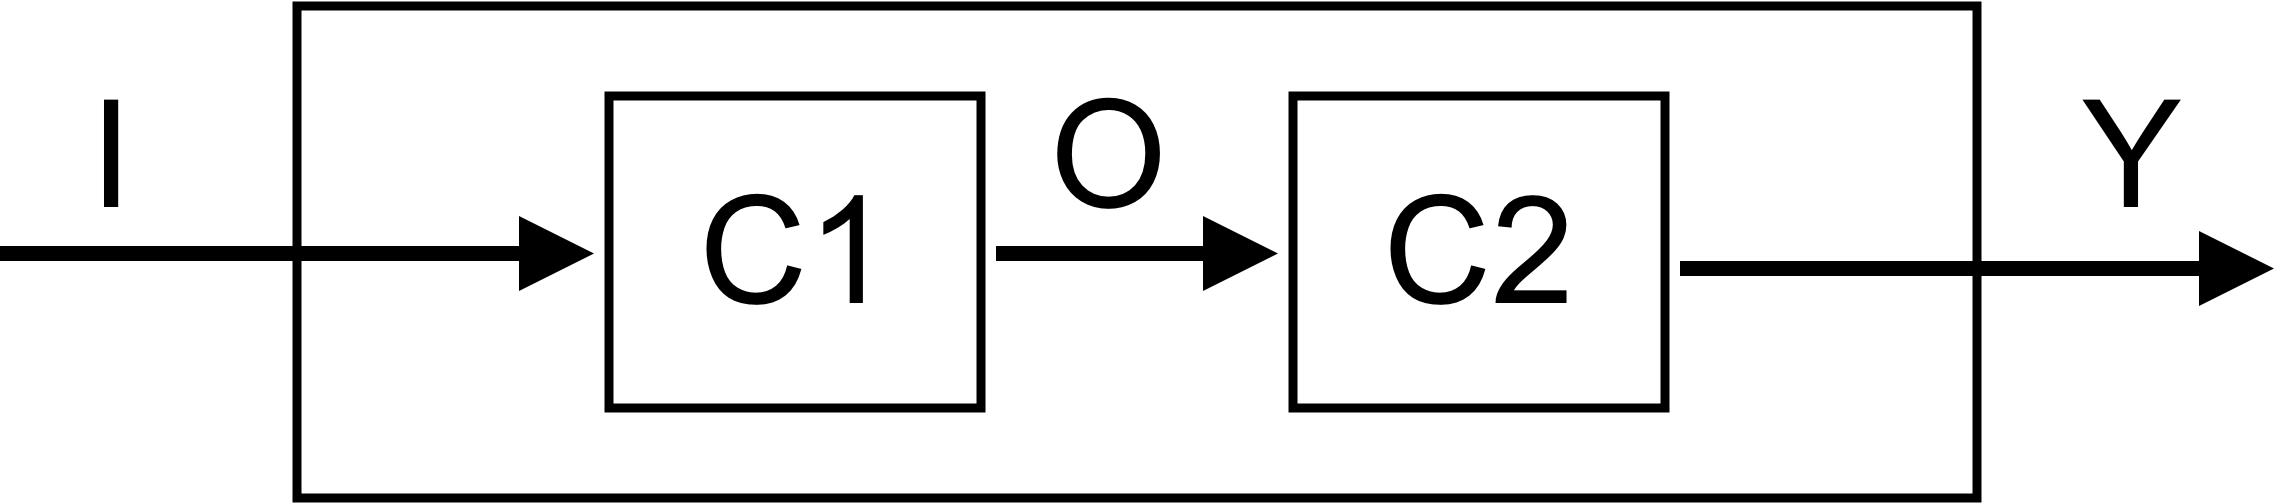
\includegraphics[width=0.4\textwidth]{figures/API-concat-operator.png}
	\end{center}
	\caption{Linear composition operator \code{concat}}
	\label{fig:concat-operator}
\end{figure}

It should be clear by now that given a value of type \code{I}, component \code{c1} should transform this into a value\footnote{Notice that the transformation in \code{c1} can also cause the output to return multiple values over time or no values at all.} of type \code{O}. This value is then used as the input of component \code{c2}, which in turn transforms it into a value of type \code{Y}. This value is then emitted as the output of the composed component. Besides these \code{OnNext} events, the \obs in either component can return an \code{OnError} or \code{OnCompleted} event. In this case the component not only has to propagate these events to the next component, but also needs to signal upstream that it is terminating. This means that the \subj which is inside the \comp can unsubscribe itself from every observer, and do this for all upstream components as well.

The behavior for regular \code{OnNext} events can be achieved by connecting the various streams in \Cref{fig:concat-operator} by subscribing them to each other. Notice that we have to connect the components in reversed order; that is, first subscribe the output of \code{c2} to the output of the composed component, then subscribe the output of \code{c1} to the input of \code{c2} and finally subscribe the input of the composed component to the input of \code{c1}. The reason for this is that either \code{c1} or \code{c2} might have elements that emit immediately when the stream is subscribed. Due to the nature of a \subj, these events would get lost if the \comp did not yet subscribe its output to something else.

The behavior of the terminal events can be achieved by using the functionality of Rx to compose subscriptions. In RxMobile every \obv is a \subs as well and likewise every \comp is an \obv, so we just need to \textit{add} the subscriptions to each other. To do so, we also require the subscription that represents the output of the \comp to be created. We get this by creating a new \obs and using the \obv in the lambda expression for this.

\begin{minipage}{\linewidth}
\begin{lstlisting}[style=ScalaStyle, caption={Linear composition operator \code{concat}}, label={lst:concat-operator}]
implicit class Operators[I, O](val src: Component[I, O]) {
  def concat[Y](other: Component[O, Y]): Component[I, Y] $=$ {
    val result $=$ Component[I, Y](input $\Rightarrow$ Observable.create(output $\Rightarrow$ {
      other.asObservable.subscribe(output)
      src.asObservable.subscribe(other)
      input.subscribe(src)

      output $+=$ other
      other $+=$ src
    }))
    src $+=$ result
    result
  }
}
\end{lstlisting}
\end{minipage}

\subsubsection{Abstracting over composition}
As we will use this feature of combining the \subs with the \comp to be created, we will already abstract over this and use this in upcoming operators as well.

\begin{minipage}{\linewidth}
\begin{lstlisting}[style=ScalaStyle, caption={\code{lift} operator}, label={lst:lift-operator}]
def lift[X, Y](f: (Observable[X], Observer[Y])$\Rightarrow$Unit): Component[X, Y] $=$ {
  val result $=$ Component[X, Y](input $\Rightarrow$ Observable.create(f(input, _)))
  src $+=$ result
  result
}
\end{lstlisting}
\end{minipage}

We can then use \code{lift} in \code{concat} as follows:

\begin{minipage}{\linewidth}
\begin{lstlisting}[style=ScalaStyle, caption={Revised implementation of the \code{concat} operator}, label={lst:concat-revised}]
implicit class Operators[I, O](val src: Component[I, O]) {
  def concat[Y](other: Component[O, Y]): Component[I, Y] $=$ {
    src.lift((input, output) $\Rightarrow$ {
      other.asObservable.subscribe(output)
      src.asObservable.subscribe(other)
      input.subscribe(src)

      output $+=$ other
      other $+=$ src
    })
  }
}
\end{lstlisting}
\end{minipage}

In general \code{lift} can be viewed as the creation of a new, encapsulating \comp, whose behavior is defined in the function \code{f}. The function arguments of types \obs and \obv represent the input and output of this new \comp respectively. This may seem counterintuitive at first, as a \comp has an input of type \obv and an output of type \obs. However, these types are what we see while looking at a \comp from the outside, whereas within the \code{lift} operator, we are looking at it from the inside. In that case the input has type \obs, since we want to receive new events and the output has type \obv, as we want to send new events.

\subsubsection{Formalizing the operators}
Before we continue developing new operators, we have to observe that both \code{concat} and \code{apply}/\code{create} satisfy the \textit{Arrow} type class that was described first in 2000 in a paper by John Hughes \cite{hughes2000-arrows}. The \textit{Arrow}  type class has similar operators to the \code{Monad} type class, but is defined more generally. Computations that are clearly not a monad can be composed over in the same way as computations that are a monad using this new type class. Just as a monadic type \code{M[A]} is representing a computation that delivers an \code{A}, so an arrow type \code{A[B, C]} is representing a computation with input \code{B} and output \code{C}. With that the dependence on the input of the computation is made explicit.

The \textit{Arrow} type class defines a couple of functions which are listed in \Cref{lst:arrow-typeclass} in Haskell. First of all, it defines \code{arr} to be a function that accepts a function from \code{b} to \code{c} as its input and the arrow from \code{b} to \code{c} as its output. This function is completely analogous to the \code{apply} method described earlier, where \code{b} and \code{c} are both of type \obs. Besides that, \textit{Arrow} defines the \code{(>>>)} operator, which composes two arrows together into one single arrow. Here the output of the first arrow is used as an input for the second arrow. This is of course analogue to the \code{concat} operator we just implemented. We define \code{(>>>)} as a second way of writing a linear composition.

\begin{minipage}{\linewidth}
\begin{lstlisting}[style=HaskellStyle, caption={\textit{Arrow} type class}, label={lst:arrow-typeclass}]
class Arrow a where
    arr :: (b $\rightarrow$ c) $\rightarrow$ a b c
    (>>>) :: a b c $\rightarrow$ a c d $\rightarrow$ a b d
\end{lstlisting}
\end{minipage}

\subsubsection{Parallel composition}
The careful reader may either have noticed that the definition of an arrow as provided in \Cref{lst:arrow-typeclass} is not complete or wonder how to implement an \code{add} function in arrow style. As Hughes shows, this is simple in a monadic context, but the current functions in the \textit{Arrow} type class do not satisfy the need.

\begin{lstlisting}[style=InlineHaskellStyle]
add :: Arrow a $\Rightarrow$ (a b Int) $\rightarrow$ (a b Int) $\rightarrow$ (a b Int)
add x y = $\ldots$
\end{lstlisting}

The input type \code{b} of the resulting arrow of this function needs to supply its value to both inputs of this functions arguments and combine its outputs. This is however not possible with the current \code{(>>>)} operator we have defined. Hence we require some new operators to be added to the \textit{Arrow} type class. Hughes defines these operators in terms of each other, leaving only one operator open that requires a custom implementation.

\begin{minipage}{\linewidth}
\begin{lstlisting}[style=HaskellStyle, caption={\textit{Arrow} type class}, label={lst:arrow-typeclass-full}]
class Arrow a where
    arr :: (b $\rightarrow$ c) $\rightarrow$ a b c
    (>>>) :: a b c $\rightarrow$ a c d $\rightarrow$ a b d
    first :: a b c $\rightarrow$ a (b,d) (c,d)
    
    second :: a b c $\rightarrow$ (d,b) (d,c)
    second f = arr swap >>> first f >>> swap
      where swap (x,y) = (y,x)
      
    (***) :: a b c $\rightarrow$ a d e $\rightarrow$ a (b,d) (c,e)
    f *** g = first f >>> second g
    
    (&&&) :: a b c $\rightarrow$ a b d $\rightarrow$ a b (c,d)
    f &&& g = arr ($\lambda$b $\rightarrow$ (b,b)) >>> (f *** g)
\end{lstlisting}
\end{minipage}

The operator \code{first} takes an arrow from \code{b} to \code{c} as its argument and just adds an extra input and output to the resulting arrow. \code{second} does the same, but effectively in reverse, by putting the extra input and output in the first slot. Note how it is possible to implement \code{second} in terms of \code{first} by doing extra swaps of the arguments.

\begin{figure}[H]
	\centering
	\begin{subfigure}[b]{0.35\linewidth}
		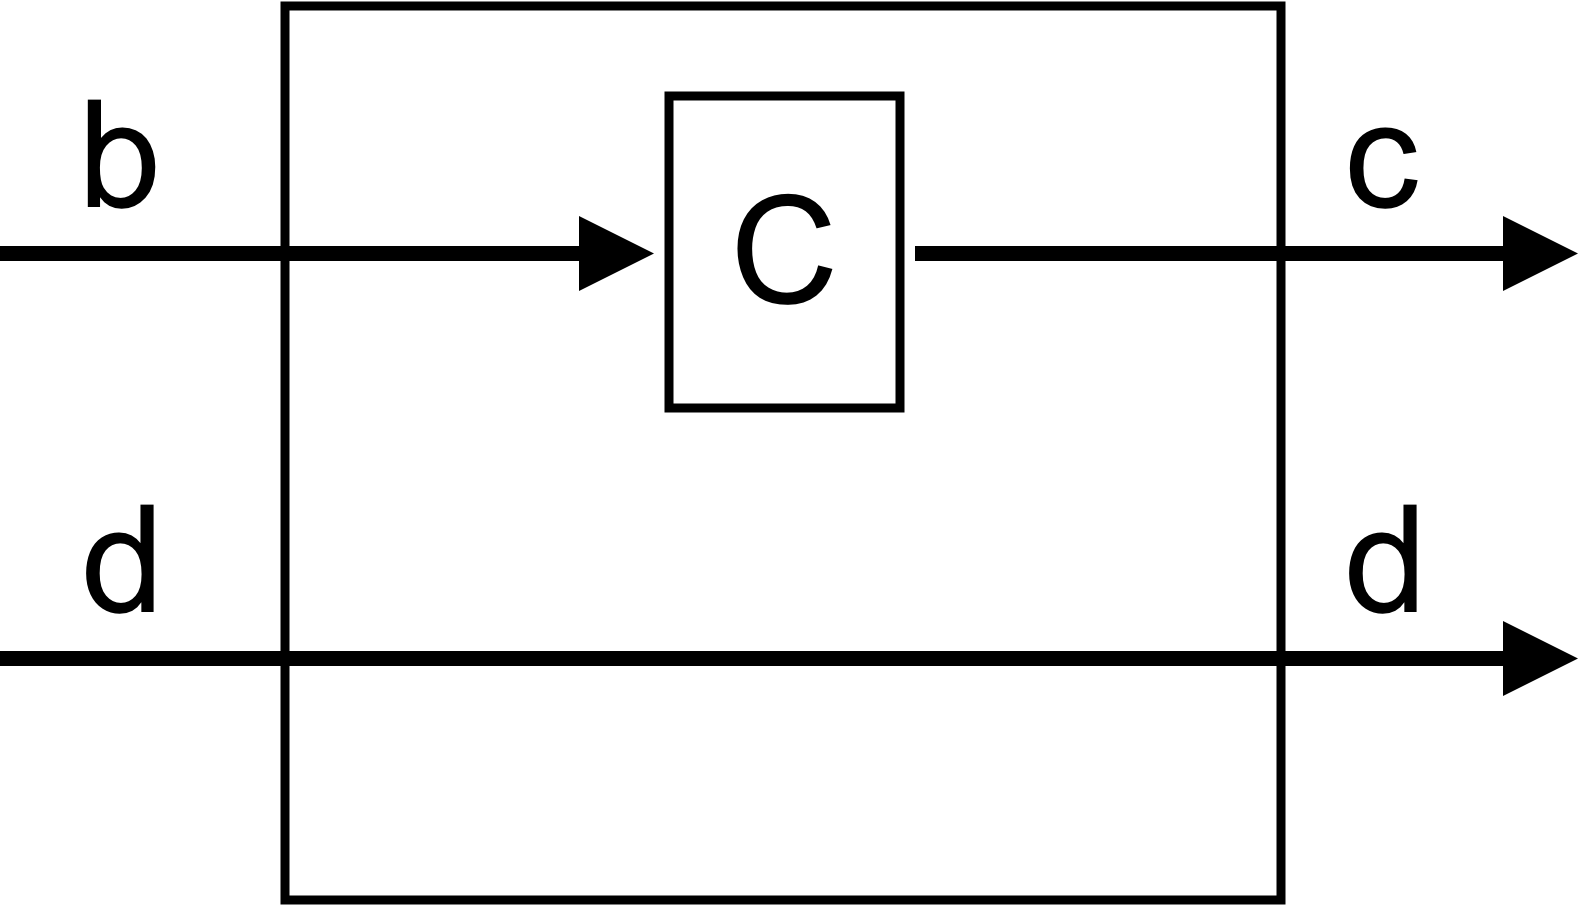
\includegraphics[width=\linewidth]{figures/API-first-operator.png}
		\caption{\code{first}}
		\label{fig:first-operator}
	\end{subfigure}
	\begin{subfigure}[b]{0.35\linewidth}
		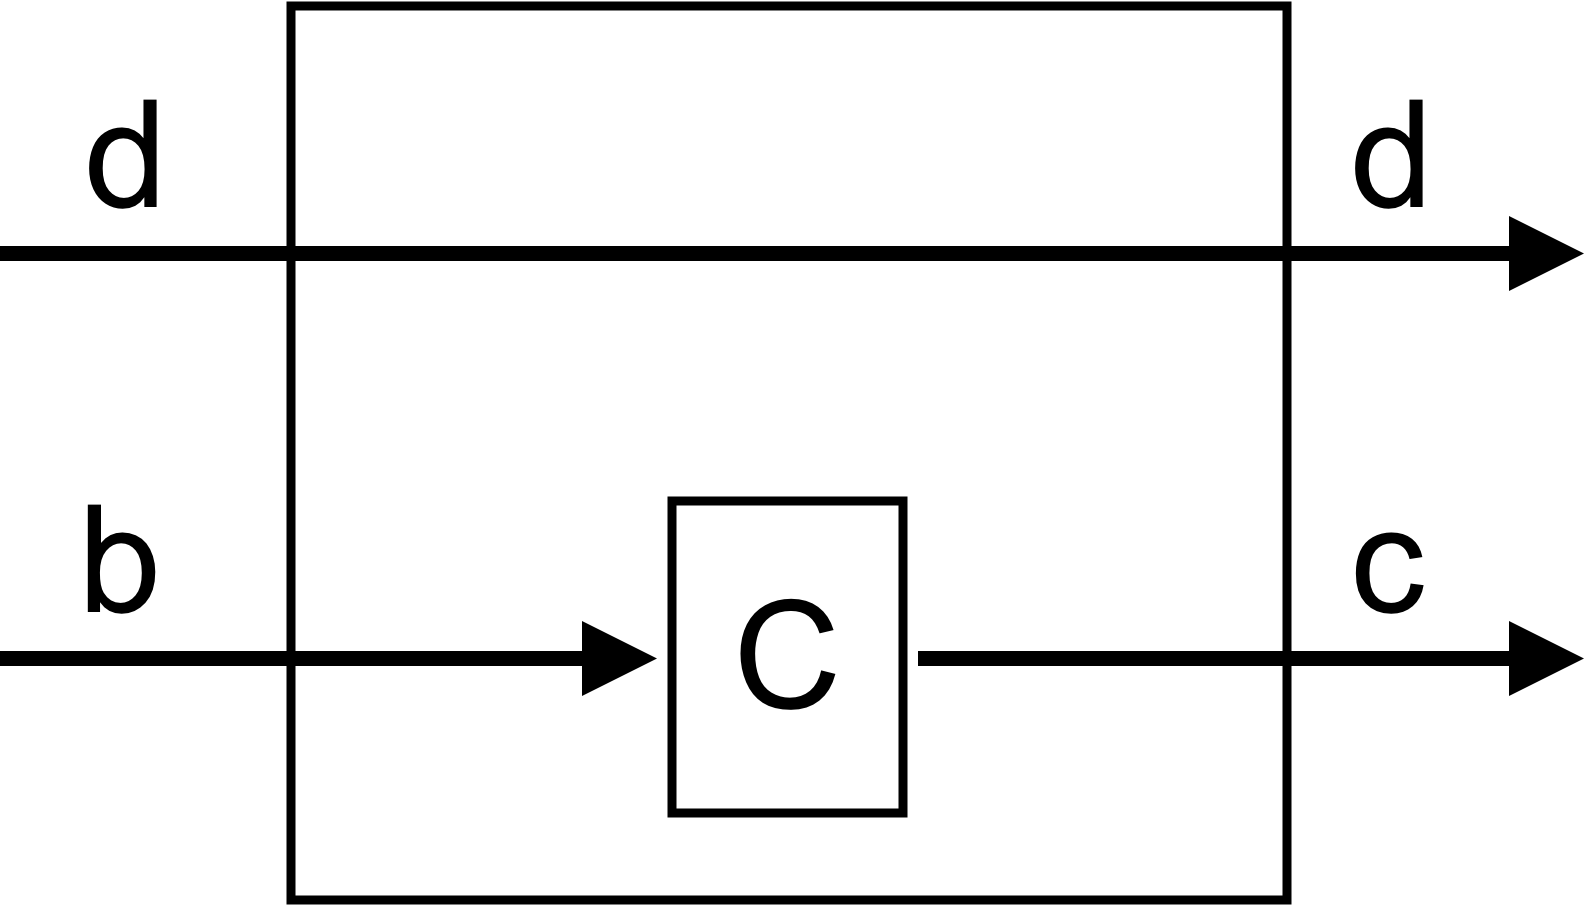
\includegraphics[width=\linewidth]{figures/API-second-operator.png}
		\caption{\code{second}}
		\label{fig:second-operator}
	\end{subfigure}
	
	\begin{subfigure}[b]{0.35\linewidth}
		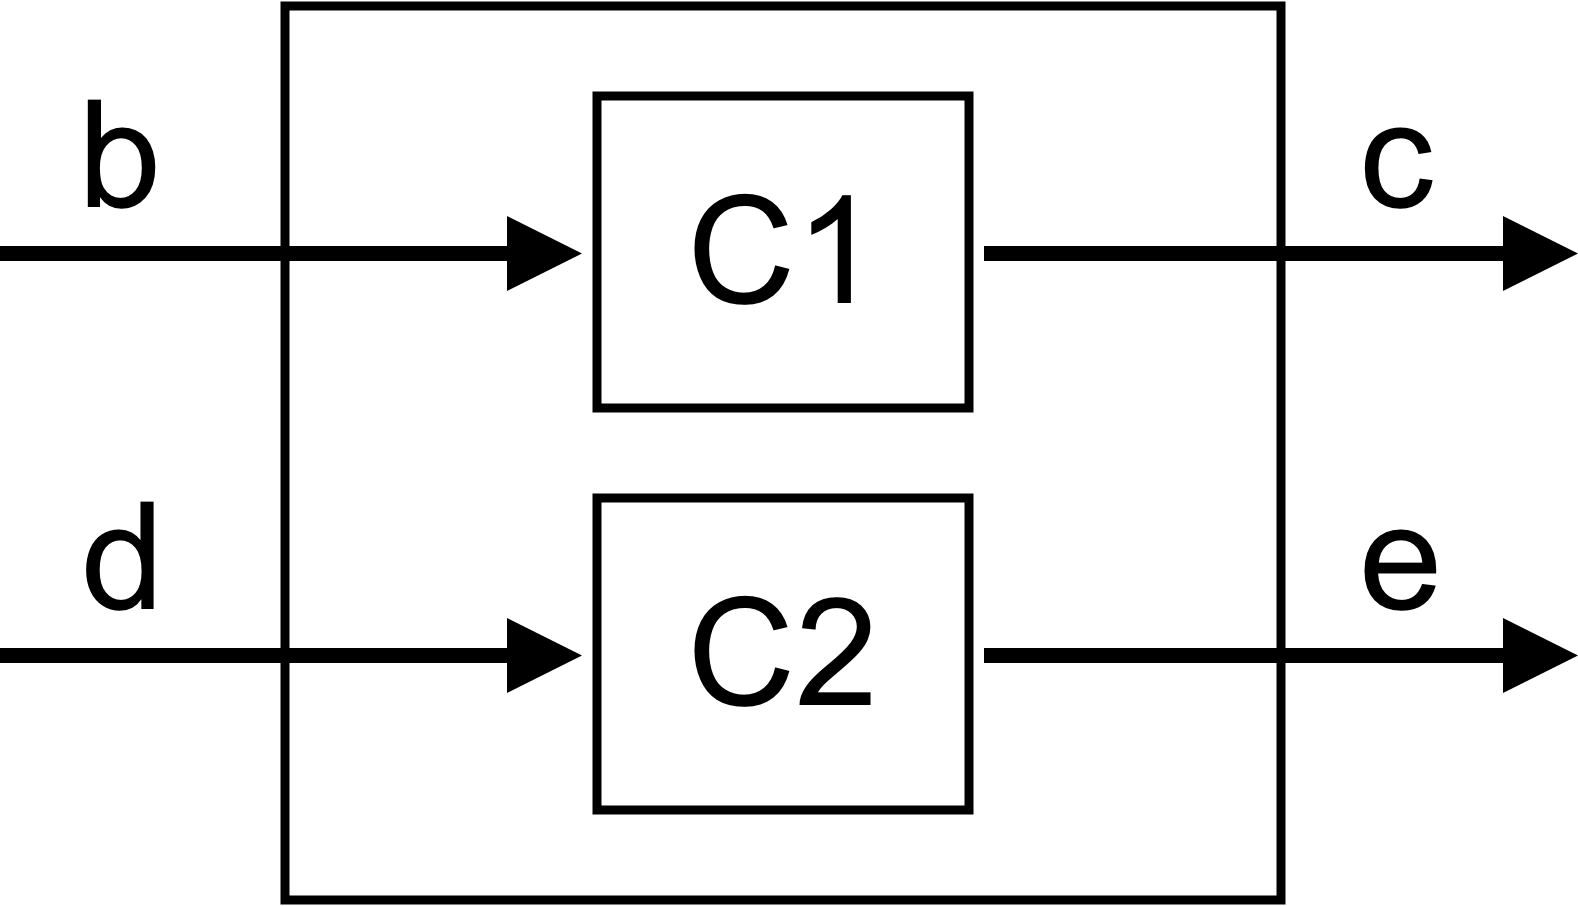
\includegraphics[width=\linewidth]{figures/API-split-operator.png}
		\caption{\code{(***)} or \code{split}}
		\label{fig:split-operator}
	\end{subfigure}
	\begin{subfigure}[b]{0.35\linewidth}
		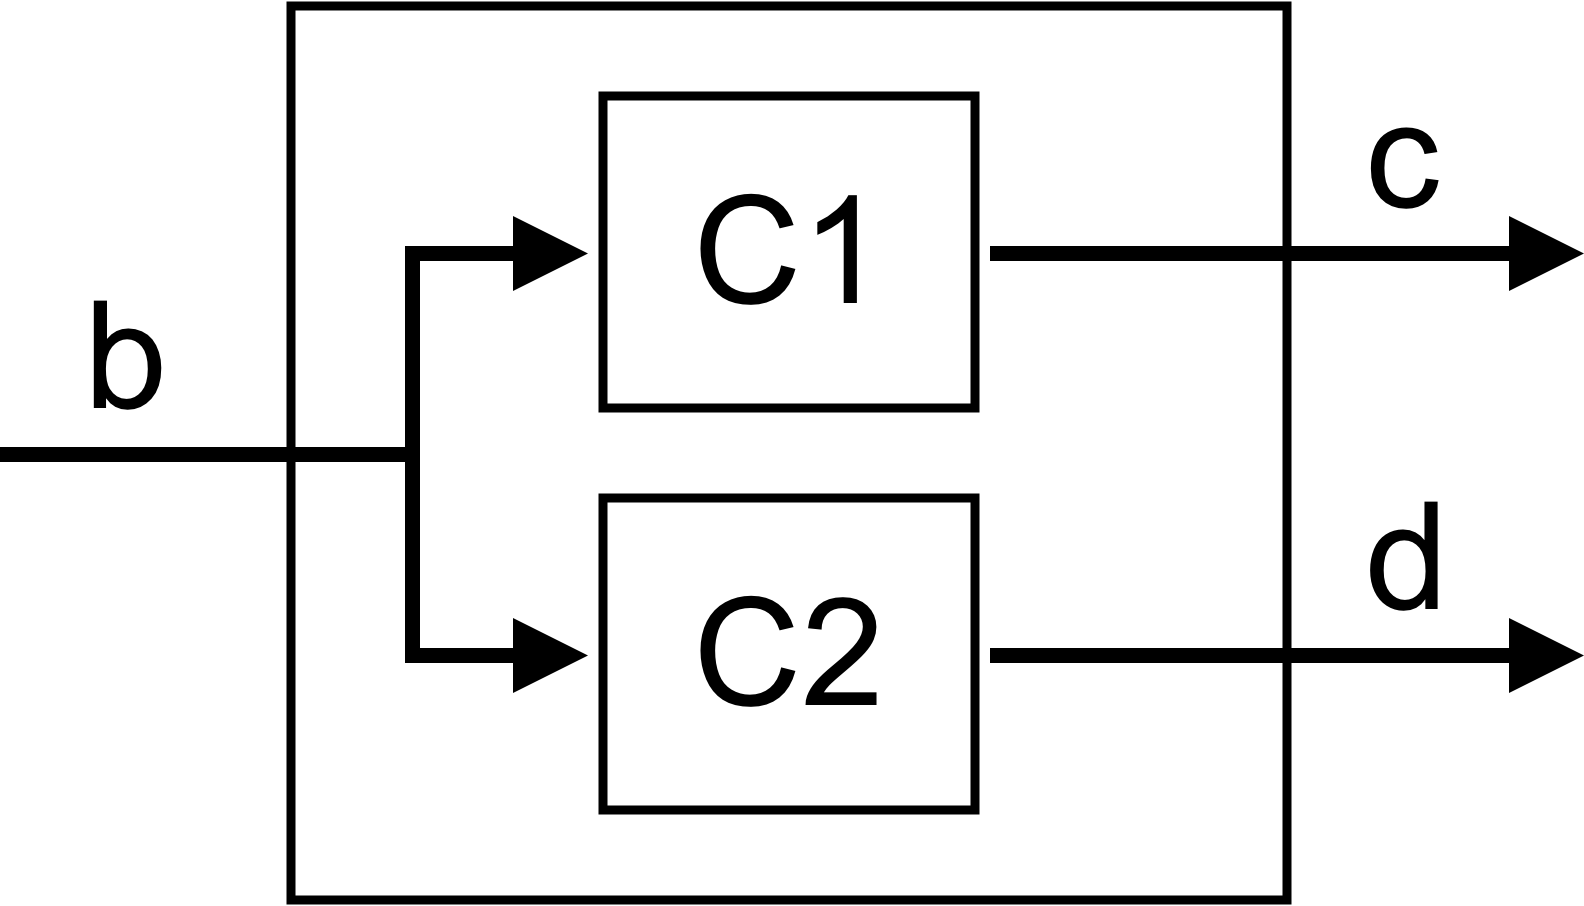
\includegraphics[width=\linewidth]{figures/API-fanout-operator.png}
		\caption{\code{(\&\&\&)} or \code{fanout}}
		\label{fig:fanout-operator}
	\end{subfigure}
	\caption{Parallel composition operators}
	\label{fig:parallel-composition}
\end{figure}

Implementing these two operators for \comp requires us to split the `\textit{input tuple stream}', apply the given \comp to the first part of this stream and merge it back with the second part of the stream. However, remember that for \obs there are a number of distinct operators for merging streams, each having their own behavior: \code{flatMap}, \code{combineLatest}, \code{withLatestFrom}, \code{zip}, \code{merge}, \code{concat}, etcetera. Since we want to merge the \comp's output stream and the second part of the input stream one-by-one, the \code{zip} operator is required here. The rest of the implementation details are just straightforward, using the earlier defined \code{lift} and taking care of the required subscriptions.

\begin{minipage}{\linewidth}
\begin{lstlisting}[style=ScalaStyle, caption={Implementations of the \textit{Arrow}'s \code{first} and \code{second} operators}, label={lst:first-and-second}]
implicit class Operators[I, O](val src: Component[I, O]) {
  $\ldots$

  def first[Y]: Component[(I, Y), (O, Y)] $=$ {
    src.lift((input, downstream) $\Rightarrow$ {
      val srcOut $=$ src.asObservable
      val inputOut $=$ input.map(_._2)

      input.map(_._1).subscribe(src)
      srcOut.zipWithBuffer(inputOut)((_, _)).subscribe(downstream)

      downstream $+=$ src
    })
  }

  def second[Y]: Component[(Y, I), (Y, O)] $=$ {
    Component.create[(Y, I), (I, Y)](_.swap) >>> src.first >>> Component.create(_.swap)
  }
}
\end{lstlisting}
\end{minipage}

The other two operators that Hughes defines for the \textit{Arrow} type class are \code{(***)} and \code{(\&\&\&)}. The former operator is used in ``\textit{parallel composition}'' of arrows, taking its input consisting of two arrows and merging them into one arrow of tuples. This is done by applying \code{first} to the first input argument and \code{second} to the second. The latter operator, takes this behavior one step further by specifying that the input type of both input arrows must be the same. With this we can construct a resulting arrow that has an input type \code{b}, whose values are supplied to both arrows, and an output type which is the tuple (or product) of both arrow's results. This type of composition is sometimes referred to as ``\textit{fanout composition}''. Implementations of these operators in the context of \comp are equivalent to the ones in \Cref{lst:arrow-typeclass-full}:

\begin{minipage}{\linewidth}
\begin{lstlisting}[style=ScalaStyle, caption={Implementations of the \textit{Arrow}'s \code{(***)} and \code{(\&\&\&)} operators}, label={lst:parallel-and-fanout}]
implicit class Operators[I, O](val src: Component[I, O]) {
  $\ldots$

  def ***[X, Y](other: Component[X, Y]): Component[(I, X), (O, Y)] $=$ {
    src.first[X] >>> other.second[O]
  }

  def &&&[Y](other: Component[I, Y]): Component[I, (O, Y)] $=$ {
    Component.create[I, (I, I)](b $\Rightarrow$ (b, b)) >>> (src *** other)
  }
}
\end{lstlisting}
\end{minipage}

Using these new operators, we are now able to define the \code{add} function in arrow style as described above. We compose the two arrows using a fanout and bring the two results together by using another component that adds the two values together. Notice that this function would be particularly interesting when implementing a PID controller or any other parallel composed set of components.

\begin{lstlisting}[style=InlineHaskellStyle]
add :: Arrow a $\Rightarrow$ (a b Int) $\rightarrow$ (a b Int) $\rightarrow$ (a b Int)
add x y = (x &&& y) >>> arr ($\lambda$(b,c) $\rightarrow$ b + c)
\end{lstlisting}

Hughes finishes this trail by generalizing the \code{add} to a \code{liftA2}, which is equivalent in functionality to Haskell's \code{liftM2} which combines the results of two monadic computations. Besides two input arrows, \code{liftA2} accepts a combinator function that is applied after the fanout composition of the two arrows. We define a similar operator called \code{combine} in our API for the purpose of parallel composition:

\begin{minipage}{\linewidth}
\begin{lstlisting}[style=ScalaStyle, caption={Implementation of the \code{Arrow}'s \code{liftA2} or \code{combine} operator}, label={lst:combine-operator}]
implicit class Operators[I, O](val src: Component[I, O]) {
  $\ldots$

  def combine[X, Y](other: Component[I, X])(combiner: (O, X) $\Rightarrow$ Y): Component[I, Y] $=$ {
    (src &&& other) >>> Component.create(combiner.tupled)
  }
}
\end{lstlisting}
\end{minipage}

\subsubsection{Problems with parallel composition on \comp}
Although our implementation of these parallel composition operators in the context of \comp might seem fine at first glance, the observant reader might have spotted some flaws in it. The main concern here is the choice of using \code{zip} in the \code{first} operator. As discussed in section \Cref{sec:fastproc-slowcons}, \code{zip} is particularly risky to use given the unpredictable nature of its source streams. This same danger comes up in our implementation of \code{first}, as the inner component might produce more than one element for every received element or as it might start with a certain number of elements before producing elements based on what it receives\footnote{This can be achieved using \code{startWith}, which is a well-known operator for \obs and which we will introduce later in the context of \comp.}.

Besides that, given that \code{zip} is used in the \code{first} operator, it follows that it is also used in \code{second} and that it is technically used twice in \code{(***)}, \code{(\&\&\&)} and \code{combine}. This is not only twice as risky, but is also fairly inefficient as the underlying Rx code needs to maintain two queues now. We will show that this can be done more efficiently by reducing the uses of \code{zip} to only once per \code{combine} operation.

For this we have to observe that we can not only implement \code{(***)} in terms of \code{first} and \code{second} but that it is also possible to implement both \code{first} and \code{second} in terms of \code{(***)}! After all, \code{first} is completely equal to \code{(***)} with the second input arrow being the identity. We can easily see this by comparing \Cref{fig:first-operator} to \Cref{fig:split-operator} where \code{c2} is equal to \code{Component.identity}. The same is true for \code{second} by making \code{c1} in \Cref{fig:split-operator} the identity \comp.

The \code{(***)} operator can then be implemented in terms of \code{lift} by splitting the input stream and subscribing both parts to the first and second component respectively. Then the outputs of these components are zipped together into a tuple and subscribed to the output of the resulting \comp. After that we are only left with some administrative work in terms of the subscriptions.

The other operators, \code{(\&\&\&)} and \code{combine} do not require any modifications as they were already implemented in terms of \code{(***)}. The full implementation of the parallel composition operators in our API now looks as follows:

\begin{minipage}{\linewidth}
\begin{lstlisting}[style=ScalaStyle, caption={New implementation of the \textit{Arrow}'s operators}, label={lst:new-arrow-implementation}]
implicit class Operators[I, O](val src: Component[I, O]) {
  $\ldots$

  def first[Y]: Component[(I, Y), (O, Y)] $=$ {
    src *** Component.identity[Y]
  }

  def second[Y]: Component[(Y, I), (Y, O)] $=$ {
    Component.identity[Y] *** src
  }

  def ***[X, Y](other: Component[X, Y]): Component[(I, X), (O, Y)] $=$ {
    src.lift((input, downstream) $\Rightarrow$ {
      input.map(_._1).subscribe(src)
      input.map(_._2).subscribe(other)

      src.asObservable.zipWithBuffer(other.asObservable)((_, _)).subscribe(downstream)

      downstream $+=$ src
      downstream $+=$ other
    })
  }

  def &&&[Y](other: Component[I, Y]): Component[I, (O, Y)] $=$ {
    Component.create[I, (I, I)](b $\Rightarrow$ (b, b)) >>> (src *** other)
  }

  def combine[X, Y](other: Component[I, X])(combiner: (O, X) $\Rightarrow$ Y): Component[I, Y] $=$ {
    (src &&& other) >>> Component.create(combiner.tupled)
  }
}
\end{lstlisting}
\end{minipage}

\subsubsection{Functor, Applicative, Monad}
One of the reasons that Hughes introduced the \textit{Arrow} \cite{hughes2000-arrows} is that he saw that not all kinds of computations can be described in terms of monads. He uses the parser library by Swierstra and Duponcheel \cite{swierstra1996-parsers} as an example of a structure that can implement the choice combinator from the \textit{MonadPlus} type class but turns out to have no possible implementation for the \textit{Monad}'s \code{(>>=)} operator. Their solution to this problem is to discard the use of a \textit{Monad} and instead use a different operator \code{(<*>)} that later became known as part of the \textit{Applicative} type class. Nowadays \textit{Applicative} sits right in the middle between \textit{Functor} and \textit{Monad} and \textit{MonadPlus} not only `inherits' from \textit{Monad} but also from \textit{Alternative}, which already has the choice combinator (see \Cref{lst:type-classes-for-monads}).

As an alternative to introducing the \code{(<*>)} operator as Swierstra and Duponcheel did, Hughes introduces the \textit{Arrow} as the answer to combining non-monadic computations. With this he shows that every \textit{Monad} is in fact an \textit{Arrow}, but that not every \textit{Arrow} is a \textit{Monad}. For this he introduces another type class \textit{ArrowApply} (\Cref{lst:arrow-apply}), which he shows to be equivalent to the \textit{Monad} type class. From this it follows that for an \textit{Arrow} to be also a \textit{Monad} it must be able to implement the \textit{ArrowApply} type class.

\begin{lstlisting}[style=HaskellStyle, caption={\textit{ArrowApply} type class}, label={lst:arrow-apply}, captionpos=b, numbers=none]
class Arrow a $\Rightarrow$ ArrowApply a where
  app :: a (a b c, b) c
\end{lstlisting}

\begin{minipage}{0.6\linewidth}
\begin{lstlisting}[style=HaskellStyle, caption={Monadic type classes}, label={lst:type-classes-for-monads}, captionpos=b, numbers=none]
class Functor f where
  fmap :: (a $\rightarrow$ b) $\rightarrow$ f a $\rightarrow$ f b

class Functor f $\Rightarrow$ Applicative f where
  pure :: a $\rightarrow$ f a
  (<*>) :: f (a $\rightarrow$ b) $\rightarrow$ f a $\rightarrow$ f b

class Applicative m $\Rightarrow$ Monad m where
  return :: a $\rightarrow$ m a
  (>>=) :: m a $\rightarrow$ (a $\rightarrow$ m b) $\rightarrow$ m b

class Applicative f $\Rightarrow$ Alternative f where
  empty :: f a
  (<$|$>) :: f a $\rightarrow$ f a $\rightarrow$ f a

class (Alternative m, Monad m) $\Rightarrow$ MonadPlus m where
  mzero :: m a
  mzero = empty
  
  mplus :: m a $\rightarrow$ m a $\rightarrow$ m a
  mplus = (<$|$>)
\end{lstlisting}
\end{minipage}
\begin{minipage}{0.4\linewidth}
	\begin{figure}[H]
		\begin{center}
			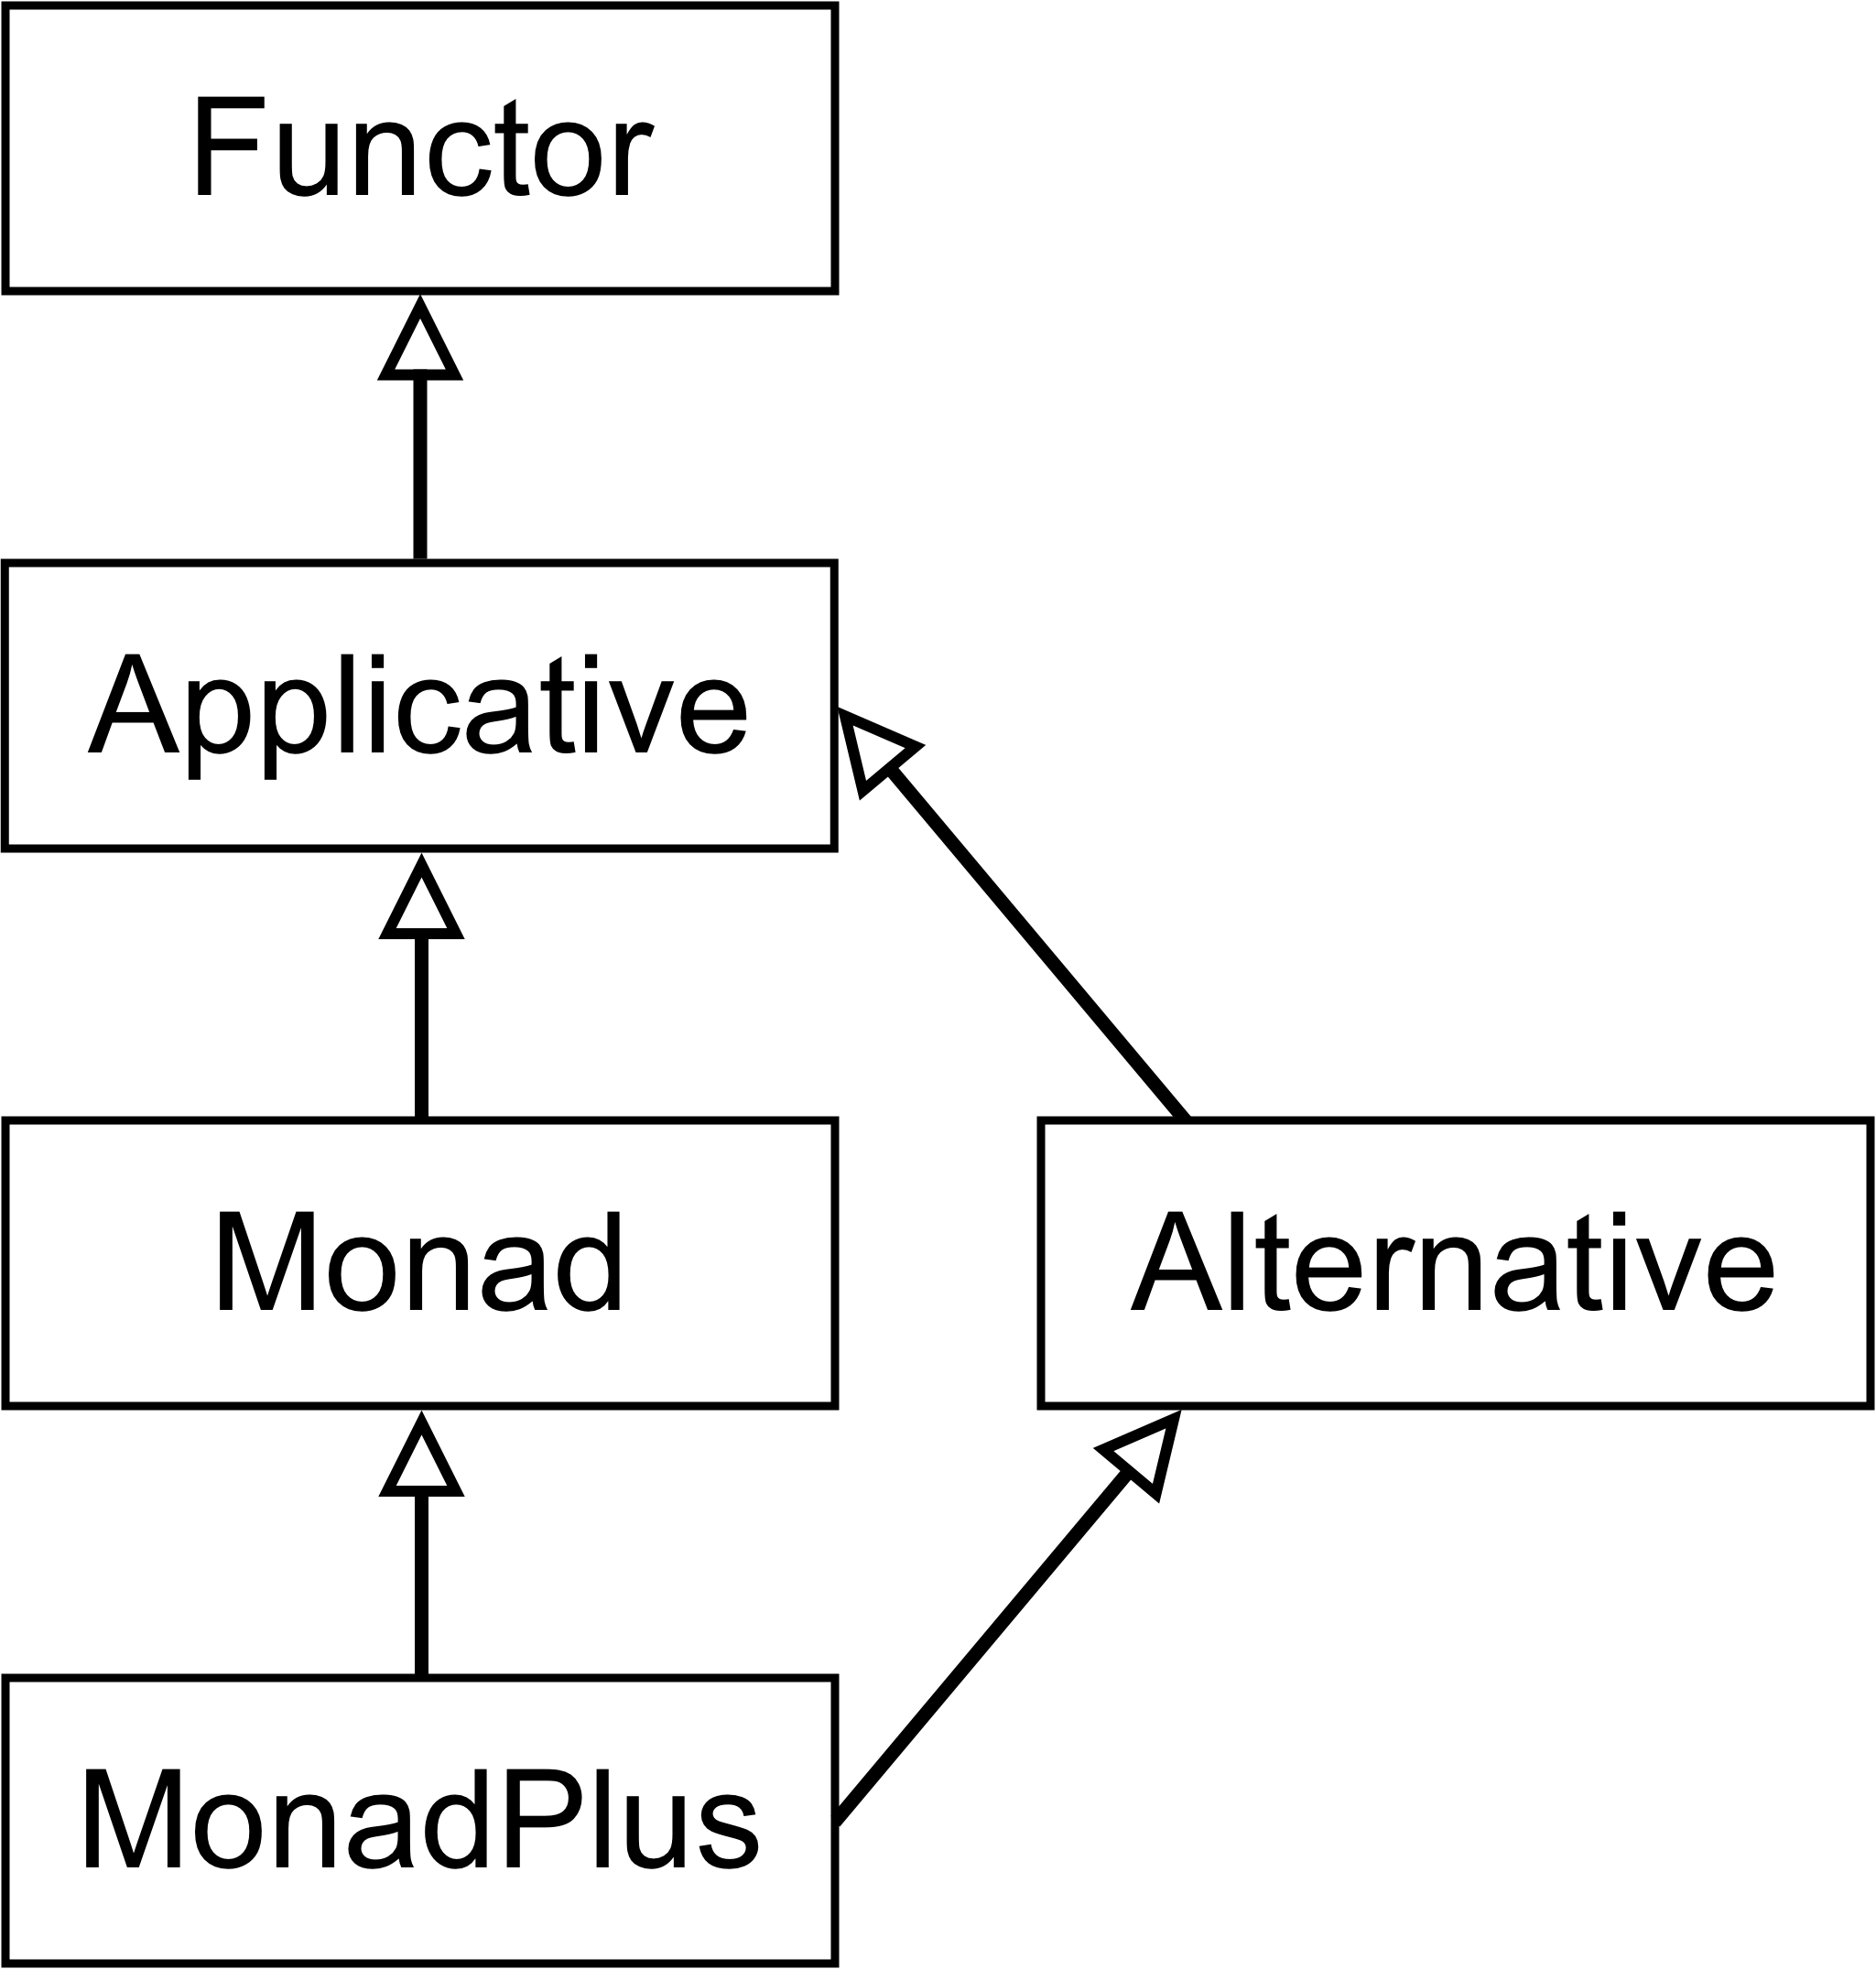
\includegraphics[width=\textwidth]{figures/Monadic-type-classes.png}
		\end{center}
		\caption{Monadic type classes}
		\label{fig:type-classes-for-monads}
	\end{figure}
\end{minipage}

In the previous sections we have demonstrated the \comp interface to be an \textit{Arrow}, which, given the discussion above, brings us to the question whether \comp is also a \textit{Functor}, \textit{Applicative} and \textit{Monad} and hence whether we are allowed to add the associated operators to our API.

The \textit{Functor} type class (\Cref{lst:type-classes-for-monads}) contains a single function \code{fmap} which accepts a \textit{Functor} and a function as its input and returns a new \textit{Functor} on which the function is applied. Translated to the \comp interface, \code{map}\footnote{\code{fmap} in Haskell is usually referred to in Scala as \code{map}} applies a transformation function to the output of the given \comp. This is simple, as we can already wrap a function in a \comp using the \code{create} operator and we can concatenate two components using \code{concat} or \code{(>>>)}.

The \textit{Applicative} type class (\Cref{lst:type-classes-for-monads}) contains two functions, \code{pure} and \code{(<*>)}. We already have the former function in our API, namely \code{from} (\Cref{lst:creating-component}). The latter function is almost the same as \code{fmap}, only with the difference that the function is wrapped inside an \textit{Applicative}. The two input parameters of \code{(<*>)} need to be merged into a single \textit{Applicative} where the function from the first parameter is applied to the value from the second parameter. We also already have this functionality in the form of the \code{combine} operator, which combines two instances of \comp using a given function.

\begin{minipage}{\linewidth}
\begin{lstlisting}[style=ScalaStyle, caption={\textit{Functor} and \textit{Applicative} operators}, label={lst:functor-and-applicative}]
implicit class Operators[I, O](val src: Component[I, O]) {
  $\ldots$

  def map[X](f: O $\Rightarrow$ X): Component[I, X] $=$ src >>> Component.create(f)
  
  def <*>[X, Y](other: Component[I, X])(implicit ev: O $<:<$ (X $\Rightarrow$ Y)): Component[I, Y] $=$ {
    src.combine(other)(ev(_)(_))
  }
}
\end{lstlisting}
\end{minipage}

Contrary to the previous type classes, it turns out that we are not able to implement the \textit{Monad}'s \code{(>>=)} (or \code{flatMap}) operator. Note that this is equivalent to saying that we are unable to implement the \textit{ArrowApply}'s \code{app} operator. Writing down these definitions shows how non-sensible both these definitions are:

\begin{lstlisting}[style=InlineScalaStyle]
implicit class MonadOperators[I, O](val src: Component[I, O]) {
  def flatMap[X](f: O $\Rightarrow$ Component[I, X]): Component[I, X]
  def app(implicit ev: I $<:<$ (Component[I, O], I)): Component[I, O]
}
\end{lstlisting}

From the perspective of \code{flatMap} it would mean that every time \code{src} produces an output, it is fed to the function \code{f}, which would produce a completely new \comp to be subscribed to the result of \code{flatMap}. This would mean that after $n$ outputs, there are $n$ \comp which are `dynamically' created and that the resulting component will emit $n$ values. The same holds for \code{app}, which would receive a new \comp to invoke with every input it receives.

The fact that \comp is not a monad may seem surprising at first, but is actually supported by Hughes, who gives an example of stream processing (which is similar in behavior to our API, but very different in its implementation) and also concludes that stream processing cannot be fitted into the monadic framework \cite{hughes2000-arrows}. He concludes that this is again an example of why not every instance of an \textit{Arrow} type class is automatically a \textit{Monad} as well.

\subsubsection{Reactive operators}
Since the \comp interface is written in terms of Rx, we may also want to use some of the operators that are defined on \obs. For example, a components may be a filter or just the functionality that it will skip the first $n$ elements it receives or start by emitting a certain value before responding to the \comp's actual input.

One way of doing this would be to create new components for each of these operations as they are needed while writing the feedback system and performing linear composition on these components. However, this would reduce the expressiveness and readability of the program that is written and would mean a lot of repeats of the same code: \code{x >>> Component(\char`_.$operator1$) >>> Component(\char`_.$operator2$)}.

A better way of doing this would be to add the most commonly used operators to the \comp API. By doing so, we can eliminate writing a lot of the same code, make the API more pleasant to use and improve the readability of the code. In fact, we have already introduced one operator that is also an operator in the Rx libraries and follows the implementation pattern as shown above: \code{map} (\Cref{lst:functor-and-applicative}).

Because the implementations of these operators will be almost identical in every case, we first introduce an operator \code{liftRx} (\Cref{lst:rx-style-operators}), which lifts an Rx operator into the \comp API such that it can be used in the API as a proper operator. This not only serves the purpose of eliminating duplicate code in the API but can also be used to have a way of lifting an Rx operator that is not present in our API.

Some of the operators present in the API are listed in \Cref{lst:rx-style-operators}, though many more can be thought of to be added.

\begin{minipage}{\linewidth}
\begin{lstlisting}[style=ScalaStyle, caption={Rx style operators}, label={lst:rx-style-operators}]
implicit class Operators[I, O](val src: Component[I, O]) {
  $\ldots$

  def liftRx[Y](f: Observable[O] $\Rightarrow$ Observable[Y]) $=$ src >>> Component(f)
  
  def drop(n: Int): Component[I, O] $=$ liftRx(_.drop(n))
  def filter(predicate: O $\Rightarrow$ Boolean): Component[I, O] $=$ liftRx(_.filter(predicate))
  def map[X](f: O $\Rightarrow$ X): Component[I, X] $=$ liftRx(_.map(f))
  def sample(interval: Duration, scheduler: Scheduler $=$ NewThreadScheduler()) $=$ liftRx(_.sample(interval, scheduler))
  def startWith(o: O): Component[I, O] $=$ liftRx(_.startWith(o))
  def scan[Y](seed: Y)(combiner: (Y, O) $\Rightarrow$ Y): Component[I, Y] $=$ liftRx(_.scanLeft(seed)(combiner))
  def take(n: Int): Component[I, O] $=$ liftRx(_.take(n))
  def throttle(duration: Duration, scheduler: Scheduler $=$ NewThreadScheduler()) $=$ liftRx(_.throttle(duration, scheduler))
}
\end{lstlisting}
\end{minipage}

Given these new operators, we can reimplement the \code{RunningAverage} example from \Cref{lst:running-average-final}. As all will agree, this looks much better and makes the code more readable and usable!

\begin{minipage}{\linewidth}
\begin{lstlisting}[style=ScalaStyle, caption={Implementation of \code{RunningAverage} using the new Rx style operators}, label={lst:running-average-with-operators}]
implicit class RunningAverageOperator(val src: Component[Double, Double]) {
  def runningAverage: Component[Double, Double] $=$ {
    src.scan(new Queue[Double]) { case (queue, value) $\Rightarrow$
        if (queue.length $==$ n)
          queue.dequeue()
        queue $+=$ value
      }
      .drop(1)
      .map(queue $\Rightarrow$ queue.sum / queue.size)
  }
}
\end{lstlisting}
\end{minipage}

\subsubsection{Feedback operator}
One of the most needed operations in building feedback systems is \textit{feedback}; the notion of feeding back a \comp's output to its input after merging it with the latest element of another stream, while also emitting the same output to the surrounding \comp (see \Cref{fig:feedback-operator}).

Though this may seem easy given the infrastructure that we have already build around our API, using \code{lift} and subscriptions, there are some technicalities that need to be taken into account in this implementation. First of all, in this situation there is a kind of recursion involved on the stream level. This needs some work as the recursed values' emissions need to be postponed to the appropriate moment rather than being emitted directly. Besides that, although the expected behavior of merging a \comp with \code{setpoint} can be naively implemented using a \code{withLatestFrom}, it turns out that this does not work in the case where \code{setpoint} emits its \emph{only} element before the \comp emits anything. This has to do with the behavior of \code{withLatestFrom} which discards everything that is emitted on the second \obs as long as the first \obs has not yet emitted any values.

The first concern, regarding the recursion, is solvable with the dedicated \code{TrampolineScheduler} which is available in both RxJava and RxMobile. This scheduler is specially created for recursive streams like this one and ``\textit{queues work on the current thread to be executed after the current work completes}'' \cite{RxJava-Trampoline-Scheduler}. As long as the stream that runs back into the input of the \comp is observed on this \sch (\Cref{lst:feedback-operator} \cref{line:observe-on-trampoline}), the recursion should work out fine.

The concern about an early emitting \code{setpoint} is somewhat harder to fix. To solve this, we have to do a \code{combineLatest} on these streams in order to not discriminate against which stream emits first. However, as soon as both streams have emitted their first value, we have to switch to the original \code{withLatestFrom} behavior. This is done in the function \code{loop} in \Cref{lst:feedback-operator} \cref{line:feedback-loop}. Here the first values of each of the two streams are merged into a tuple using the \code{combineLatest} and \code{take(1)}. Notice that the latter causes the stream to complete immediately after the first tuple is emitted. This \code{OnCompleted} is however postponed by \code{flatMap} until the inner-stream is completed. Inside the \code{flatMap} we unpack the tuple again and feed the values as the first new input of the \code{src} component. Here also the merging behavior is `replaced' by \code{withLatestFrom}. Due to our earlier concern with recursion, we have to use the extra \code{Observable.create} here and feed the first tuple to the \code{observer} by hand.

\begin{figure}[H]
	\begin{center}
		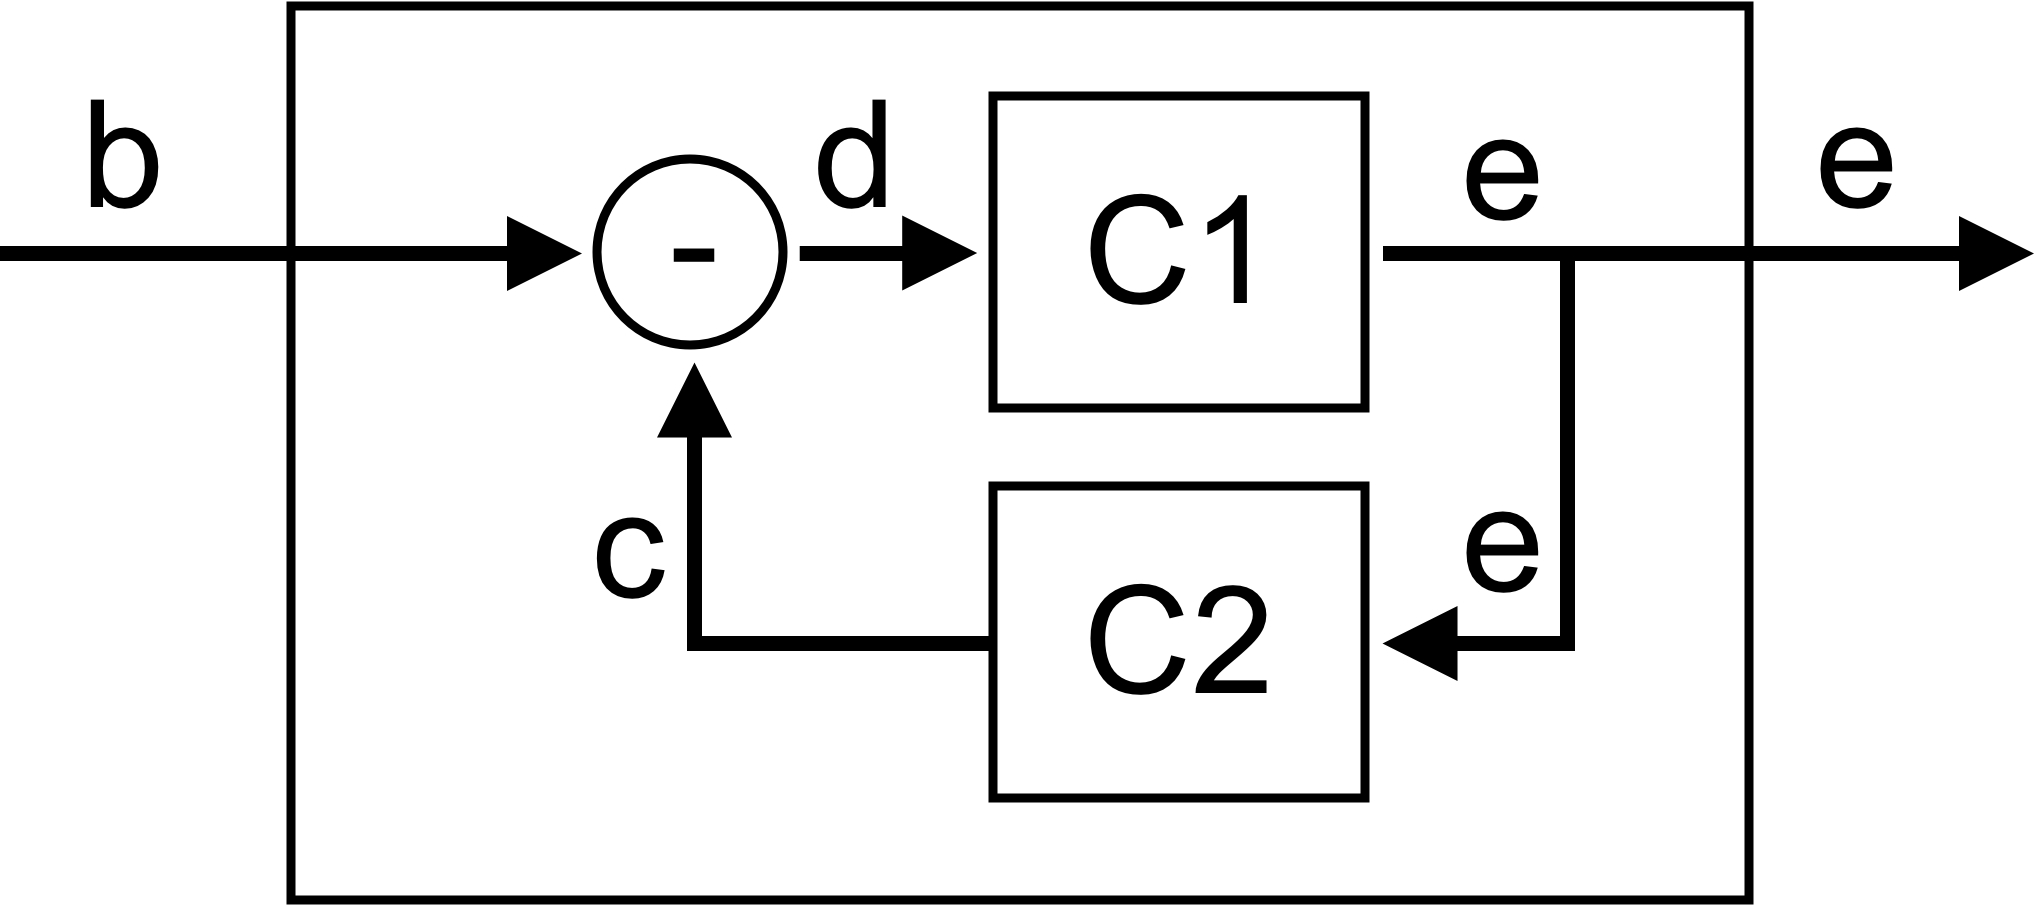
\includegraphics[width=0.4\textwidth]{figures/API-feedback-operator.png}
	\end{center}
	\caption{Feedback operator}
	\label{fig:feedback-operator}
\end{figure}

With the \code{loop} function in place, we can implement the \code{feedback} operator as shown in \Cref{lst:feedback-operator} \cref{line:feedback-operator}. As usual we use the \code{lift} operator as the basis of the implementation. Notice how we have to subscribe the output of \code{src} twice, once to the output of the encapsulating component (\code{downstream}) and once to the input of the transducer \code{trd}. Also notice that the order of subscriptions is important here: we first have to subscribe the output of the transducer to \code{src} (after applying the \code{loop} function and observing on the \code{TrampolineScheduler}) and only then subscribe the \code{src}'s output to both \code{downstream} and the transducer. Just as with \code{concat} this order of subscriptions prevents us from losing initial elements.

\begin{minipage}{\linewidth}
\begin{lstlisting}[style=ScalaStyle, caption={Feedback operator}, label={lst:feedback-operator}]
implicit class Operators[I, O](val src: Component[I, O]) {
  $\ldots$

  def feedback(f: O $\Rightarrow$ I)(implicit n: Numeric[I]): Component[I, O] $=$ {
    feedback(Component.create(f))
  }

  def feedback(tr: Component[O, I])(implicit n: Numeric[I]): Component[I, O] $=$ { |\label{line:feedback-operator}|
    lift((setpoint, downstream) $\Rightarrow$ {
      loop(tr.asObservable, setpoint)((t, s) $\Rightarrow$ n.minus(s, t))
        .observeOn(new TrampolineScheduler) |\label{line:observe-on-trampoline}|
        .subscribe(src)

      src $+=$ src.asObservable
        .publish(source $\Rightarrow$ {
          source.subscribe(downstream)
          source.subscribe(tr)

          source
        }).subscribe()

      downstream $+=$ src
      downstream $+=$ tr
      tr $+=$ src
    })
  }
  
  private def loop[T, S](transOut: Observable[T], setpoint: Observable[S]) (combinator: (T, S) $\Rightarrow$ I): Observable[I] $=$ { |\label{line:feedback-loop}|
    transOut.publish(tos $\Rightarrow$ setpoint.publish(sps $\Rightarrow$
      tos.combineLatest(sps)((_, _))
        .take(1)
        .flatMap { case (t, s) $\Rightarrow$
          Observable.create[I](observer $\Rightarrow$ {
            tos.withLatestFrom(sps.startWith(s))(combinator).subscribe(observer)
            observer.onNext(combinator(t, s))
          })
        }))
  }
}
\end{lstlisting}
\end{minipage}

With this last operator added to the API, we think we have a solid framework for creating and executing feedback systems that can be placed in production worthy systems. The interface as well as the set of operators have their foundations in theoretical concepts such as category theory and functional programming and are built on top of the very successful concept of reactive programming. It is our believe that this API can replace any imperatively created feedback system. We will use our API in \Cref{sec:reactive-balltracker} by revisiting the small \textit{ball movement control system} example from \Cref{sec:imperative-balltracker}.

\section{Improvements on the API}
The reader that is experienced with the concepts of Rx may have spotted an interesting point in the implementations of the operators in the previous section. This already becomes apparent from the implementation of \code{concat} in \Cref{lst:concat-operator,lst:concat-revised}. Although the purpose of this operator is to connect two instances of \comp in a linear composition, most of the work is spend on administrative work to subscribe streams to each other and add unsubscribe handlers. Also note again that the order in which these subscribe calls are executed is actually important!

One might argue that this is just how this operator is supposed to be set up for it to work correctly. The experienced Rx user will however respond to this by observing that all we are doing is connecting various instances of \subj in a somewhat complex manner. This is true, given the implementation of the \comp interface in \Cref{lst:component-v1}. As derived in \Cref{subsec:api-derivation}, a \comp must be an object that received elements of one type and internally transform these into another type and push out these new elements to those who are subscribed to it. Also we determined in \Cref{lst:component-v1} that the essence of \comp is the \code{transform} function which transforms a stream of elements of one type into a stream of elements of another type. This also becomes apparent in the \code{apply} function in \Cref{lst:creating-component}, which precisely has this transformation as its argument. The ceremony that is required to make this work in \Cref{lst:component-v1} involves the \subj, \obv and the associated subscription management that becomes visible in \Cref{lst:concat-operator,lst:concat-revised}.

The refactoring we propose in this section is to remove these ceremonial elements from the \comp interface and to really make the \code{transform} function the essence of the interface. For this we remove the \subj, the associated \code{\char`_subscription} value as well as the inheritance from \code{Observer[I]}. What we end up with is a simple class \comp with a \code{transform} function of type \code{Observable[I] $\Rightarrow$ Observable[O]} as its argument and in single method called \code{run} that transforms an input stream into an output stream (\Cref{lst:component-v2}). The associated \code{apply} function is changed accordingly.

\begin{minipage}{\linewidth}
\begin{lstlisting}[style=ScalaStyle, caption={Revised version of the \comp interface}, label={lst:component-v2}]
class Component[I, O](transform: Observable[I] $\Rightarrow$ Observable[O]) {

  def run(is: Observable[I]): Observable[O] $=$ transform(is)
}
object Component {
  def apply[I, O](transform: Observable[I] $\Rightarrow$ Observable[O]): Component[I, O] $=$
    new Component(transform)

  $\ldots$
}
\end{lstlisting}
\end{minipage}

Due to the way the operators are implemented we are forced to change only three of them, which we will refer to as the primative operators. These are \code{concat}, \code{(***)} and \code{feedback}. All the other operators are composed from these three operators and the \code{apply} function. The primative operators can be recognized in the previous section as those operators that were implemented in terms of \code{lift}. With the introduction of this revised version of \comp we will no longer have a need for \code{lift} and we can therefore discard this operator.  The new implementations of these primitive operators are shown in \Cref{lst:primative-operator-revisions}

\begin{minipage}{\linewidth}
\begin{lstlisting}[style=ScalaStyle, caption={Revised implementations of the primitive operators}, label={lst:primative-operator-revisions}]
implicit class Operators[I, O](val src: Component[I, O]) {
  def concat[X](other: Component[O, X]): Component[I, X] $=$
    Component(other.run _ compose src.run)
  
  def ***[X, Y](other: Component[X, Y]): Component[(I, X), (O, Y)] $=$
    Component(_.publish(ixs $\Rightarrow$ {
      src.run(ixs.map(_._1)).zipWithBuffer(other.run(ixs.map(_._2)))((_, _))
    }))
  
  def feedback(tr: Component[O, I](implicit n: Numeric[I]): Component[I, O] $=$ {
    import n._
    
    Component(setpoint $\Rightarrow$ {
      val srcIn $=$ Subject[I]()
      
      src.run(srcIn)
        .publish(out $\Rightarrow$ {
          loop(tr.run(out), setpoint)((t, s) $\Rightarrow$ s - t)
            .observeOn(new TrampolineScheduler)
            .subscribe(srcIn)

          out
        })
    })
  }
  $\ldots$
}
\end{lstlisting}
\end{minipage}

Finally we will briefly revisit the issue regarding the \comp being a \textit{Monad}. This becomes even more interesting since the \comp is now reduced to a single function. As is known from for example Haskell, the \textit{function} is considered to be a \textit{Monad}:

\begin{minipage}{\linewidth}
\begin{lstlisting}[style=InlineHaskellStyle]
instance Monad (($\rightarrow$) r) where
  return = const
  f >>= k = $\lambda$r $\rightarrow$ k (f r) r
\end{lstlisting}
\end{minipage}

Therefore we can conclude that also \comp is actually a \textit{Monad} and we must be able to write an implementation for it. However, as we have argued before, it does not make sense to make \comp into a \textit{Monad} given its context and the behavior of \code{flatMap}. Therefore we still reject \code{flatMap} as an operator in our API.

\begin{minipage}{\linewidth}
\begin{lstlisting}[style=InlineScalaStyle]
def flatMap[X](f: O $\Rightarrow$ Component[I, X]): Component[I, X] $=$ {
  Component(_.publish(is $\Rightarrow$ src.run(is).flatMap(f(_).run(is))))
}
\end{lstlisting}
\end{minipage}

The complete and final version of this API can be found in \Cref{app:feedback-api}.


\section{An extended example - revisited}
\label{sec:reactive-balltracker}
To demonstrate the intended usage of our Feedback API, we will return to the toy example developed in section \Cref{sec:imperative-balltracker} and refactor the code such that it uses the powers of both our API and Rx most optimally. The goal of this exercise (especially regarding the feedback system in this application) is to recreate \Cref{fig:balltracker-diagram} in terms of the new API and show the close resemblance between the two.

\subsection{Controller components}
First of all, we observe that in this feedback system a PID controller is present, which is, as discussed in \Cref{subsec:combining-controllers}, one of the most commonly used controllers in feedback systems. It therefore makes sense to create this controller, as well as it's separate components, and let it be part of the library we create in this chapter. This makes this controller better reusable and prevents many different implementations to be created.

Since a PID controller consists of three subcomponents, the proportional, integral and derivative control, it makes sense to first create these operators using our API. For this we will use \Cref{eq:proportional-control,eq:integral-control-discrete,eq:derivative-control} as a basis. For simplicity we will only consider integral and derivative control with a fixed $\mathrm{d} t$ value in this section, as this case applies to the Ball Movement Control example. The controllers that act on a variable $\mathrm{d} t$ value are implemented almost equally, but just with an extra \code{withLatestFrom} Rx-operator in them.

The proportional controller can be easily written as \code{Component.create(kp *)}, with \code{kp} as the proportional controller gain, and is considered too simple to be put in our library.

The integral controller can be described as a running sum over all the data the \comp receives. This is equivalent to a \code{scan} operator with a summation operator as the accumulator function. This is shown in \Cref{lst:controller-implementations}. Due to the fact that we start with an initial element that is not part of the actual data but is just a seed value, we need to discard this first element using a \code{drop(1)} operation.

The derivative controller is a little more difficult as there does not exist a dedicated operator for this in neither the Rx framework nor in our Feedback API. In the circumstances that we face in this section (fixed $\mathrm{d} t$ value), we can approximate the derivative value of a stream of values as the difference between the current and previous element. Therefore we need to use a sliding buffer followed by a pattern match that calculates the difference between them. Notice that buffer operators are not part of our API but are contained in the Rx API and we hence can use them in combination with the \code{liftRx} operator from our API. The resulting code can be found in \Cref{lst:controller-implementations}. Note that the \code{filter} operator is here because the \code{buffer} operator will produce a list with less values whenever the source stream terminates. This prevents the pattern match inside \code{map} from failing.

Finally, we can now combine these three controllers into the PI and PID controllers using the \code{combine} and \code{<*>} operators.

\begin{minipage}{\linewidth}
\begin{lstlisting}[style=ScalaStyle, caption={Implementation of the various commonly used controllers}, label={lst:controller-implementations}]
object Controllers {
  def integralController[T](ki: T)(implicit n: Numeric[T]): Component[T, T] $=$ {
    Component.identity[T]
      .scan(n.zero)(n.plus)
      .drop(1)
      .map(n.times(ki, _))
  }

  def derivativeController[T](kd: T)(implicit n: Numeric[T]): Component[T, T] $=$ {
    Component.identity[T]
      .startWith(n.zero)
      .liftRx(_.buffer(2, 1))
      .filter(_.size $==$ 2)
      .map {
        case fst :: snd :: Nil $\Rightarrow$ n.minus(snd, fst)
      }
      .map(n.times(kd, _))
  }
  
  def piController[T](kp: T, ki: T)(implicit n: Numeric[T]): Component[T, T] $=$ {
    Component.create(kp *).combine(integralController(ki))(n.plus)
  }
  
  def pidController[T](kp: T, ki: T, kd: T)(implicit Numeric[T]): Component[T, T] $=$ {
    import n._
    
    val proportional $=$ Component.create(kp *)
    val integral $=$ integralController(ki)
    val derivative $=$ derivativeController(kd)
    
    proportional.combine(integral)((p, i) $\Rightarrow$ p + i + _) <*> derivative
  }
}
\end{lstlisting}
\end{minipage}

\subsection{Ball Movement Control - refactored}
A next observation to make in our attempts to refactor the Ball Movement Control example is that the code as shown in \Cref{lst:ball-physics,lst:ball-feedback} is defined in terms of tuples to distinguish the horizontal and vertical movement. For our new implementation, however, we will separate these dimensions, write a feedback control system that applies to one-dimensional motion and combine two of these systems to get control for two-dimensional motion.

Compared to \Cref{lst:ball-physics}, we now not only have to define the position, velocity and acceleration in 2 dimensions, but also in 1 dimension (\Cref{lst:ball-physics-new}). This also holds for the \code{Ball} class, which now consists of two classes: \code{Ball1D} and \code{Ball2D}. The old \code{Ball.accelerate(Acceleration)}, which transformed an acceleration into a new position, is split into two stages, transforming an acceleration in a new velocity using \code{AccVel.accelerate} and transforming a velocity into a new position using \code{Ball1D.move}. Note that these transformations resemble the three arrows in the top middle section of \Cref{fig:balltracker-diagram}. Finally we also declare the corresponding \emph{one-dimensional} \code{BallFeedbackSystem} to be a \comp that takes positions and emits \code{Ball1D} instances. 

\begin{minipage}{\linewidth}
\begin{lstlisting}[style=ScalaStyle, caption={Ball motion physics}, label={lst:ball-physics-new}]
type Pos $=$ Double
type Vel $=$ Double
type Acc $=$ Double
type Position $=$ (Pos, Pos)
type Velocity $=$ (Vel, Vel)
type Acceleration $=$ (Acc, Acc)
type History $=$ mutable.Queue[Position]
type BallFeedbackSystem $=$ Component[Pos, Ball1D]

case class AccVel(acceleration: Acc $=$ 0.0, velocity: Vel $=$ 0.0) {
  def accelerate(acc: Acc): AccVel $=$ AccVel(acc, velocity + acc)
}

case class Ball1D(acceleration: Acc, velocity: Vel, position: Pos) {
  def move(av: AccVel): Ball1D $=$ {
    Ball1D(av.acceleration, av.velocity, position + av.velocity)
  }
}
object Ball1D {
  def apply(position: Pos): Ball1D $=$ Ball1D(0.0, 0.0, position)
}

case class Ball2D(acceleration: Acceleration, velocity: Velocity, position: Position)
object Ball2D {
  def apply(x: Ball1D, y: Ball1D): Ball2D $=$ {
    Ball2D((x.acceleration, y.acceleration), (x.velocity, y.velocity), (x.position, y.position))
  }
}
\end{lstlisting}
\end{minipage}

The next step is to translate \Cref{fig:balltracker-diagram} into an actual \code{BallFeedbackSystem} that is used instead of the imperative version in \Cref{lst:ball-feedback}.

\begin{minipage}{\linewidth}
\begin{lstlisting}[style=ScalaStyle, caption={Ball movement feedback system}, label={lst:ball-feedback-new}]
def feedbackSystem(pid: Component[Double, Acc]): BallFeedbackSystem $=$ {
  pid.map(d $\Rightarrow$ math.max(math.min(d * 0.001, 0.2), -0.2))
    .scan(new AccVel)(_ accelerate _).drop(1)
    .scan(Ball1D(ballRadius))(_ move _)
    .sample(16 milliseconds)
    .feedback(_ position)
}

def feedback: Component[Position, Ball2D] $=$ {
  val fbcX $=$ Component.create[Position, Pos](_._1) >>> feedbackSystem(pidX)
  val fbcY $=$ Component.create[Position, Pos](_._2) >>> feedbackSystem(pidY)

  fbcX.combine(fbcY)(Ball2D(_, _))
}
\end{lstlisting}
\end{minipage}


\todo{Ball Tracker example by using our API}

\begin{itemize}
	\item[\checkmark] P/I/D/PI/PID controllers as standard components
	\item the feedback system
		\begin{itemize}
			\item decouple horizontal and vertical feedback systems
			\item describe 1D feedback system (just `rewrite' the image to code!)
			\item combine feedback systems to get 2D behavior
		\end{itemize}
	\item refer to \Cref{app:ball-movement-reactive} and put the full code there.
\end{itemize}































































\clearpage
\begin{itemize}
	\item[\checkmark] Since we do feedback control for computer science, we want to come up with an API to create feedback systems
	\begin{itemize}
		\item[\checkmark] A good API does not yet exist
		\item[\checkmark] Some simple stuff in Python
		\item[\ding{55}] Solution from Peti Koch
	\end{itemize}
	\item Feedback control as ‘working with streams’
	\begin{itemize}
		\item[\checkmark] A component sits in between 2 streams and performs some sort of transformation
		\item[\checkmark] A component is compositional: connecting components, making feedback loop, zipping $\rightarrow$ a feedback system is the same as a component
		\item[\checkmark] Observation: \textbf{a component is the same as a Mealy Machine}
		\item[\checkmark] Derive the exact type of a component, starting from a Mealy Machine and using category theory
		\item[\checkmark] Observation: \textbf{a component is an Arrow}
		\item[\checkmark] Introduce the operators on Component
		\begin{itemize}
			\item[\checkmark] Concat
			\item[\checkmark] Lift (as generalizing over all operators)
			\item[\checkmark] Arrow operators (see \LaTeX code)
			\item[\checkmark] \textit{$<$many RxMobile operators$>$}
			\item[\checkmark] Feedback
		\end{itemize}
		\item[\checkmark] Second version of the API
		\begin{itemize}
			\item[\checkmark] Subjects and subscriptions are not how you work with the underlying Rx; this is not a real use case for \subj; use \obs and as few times as possible and as late as possible
			\item[\checkmark] Function \code{Observable[I] $\Rightarrow$ Observable[O]} as basis
			\item[\checkmark] Changes in operators
			\item[\checkmark] Observation: this looks like the \textit{Reader Monad} (it's a function), however, it still does not make sense for \comp to be a \textit{Monad}
		\end{itemize}
	\end{itemize}
	\item Ball tracker example with the API
\end{itemize}

\todo{below in chap4 with looking back on chap3?}
The ultimate goal in computer science (especially in software engineering) is to wrap the theory of a piece of technology in some kind of an API, such that anybody can incorperate it easily in their applications, platforms or frameworks. The notion of feedback control is however apparently so foreign to computer science that there does not exist a proper API for this yet. 